%  ========================================================================
%  Copyright (c) 1985 The University of Washington
%
%  Licensed under the Apache License, Version 2.0 (the "License");
%  you may not use this file except in compliance with the License.
%  You may obtain a copy of the License at
%
%      http://www.apache.org/licenses/LICENSE-2.0
%
%  Unless required by applicable law or agreed to in writing, software
%  distributed under the License is distributed on an "AS IS" BASIS,
%  WITHOUT WARRANTIES OR CONDITIONS OF ANY KIND, either express or implied.
%  See the License for the specific language governing permissions and
%  limitations under the License.
%  ========================================================================
%

% Documentation for University of Washington thesis LaTeX document class
% by Jim Fox
% fox@washington.edu
%
%    Revised for version 2015/03/03 of uwthesis.cls
%    Revised, 2016/11/22, for cleanup of sample copyright and title pages
%
%    This document is contained in a single file ONLY because
%    I wanted to be able to distribute it easily.  A real thesis ought
%    to be contained on many files (e.g., one for each chapter, at least).
%
%    To help you identify the files and sections in this large file
%    I use the string '==========' to identify new files.
%
%    To help you ignore the unusual things I do with this sample document
%    I try to use the notation
%       
%    % --- sample stuff only -----
%    special stuff for my document, but you don't need it in your thesis
%    % --- end-of-sample-stuff ---


%    Printed in twoside style now that that's allowed
%
 
\documentclass [11pt, proquest] {uwthesis}[2016/11/22]
 
%
% The following line would print the thesis in a postscript font 

% \usepackage{natbib}
% \def\bibpreamble{\protect\addcontentsline{toc}{chapter}{Bibliography}}

\setcounter{tocdepth}{1}  % Print the chapter and sections to the toc
 

% ==========   Local defs and mods
%

% --- sample stuff only -----
% These format the sample code in this document

\usepackage{alltt}  % 
\newenvironment{demo}
  {\begin{alltt}\leftskip3em
     \def\\{\ttfamily\char`\\}%
     \def\{{\ttfamily\char`\{}%
     \def\}{\ttfamily\char`\}}}
  {\end{alltt}}
\newenvironment{ch_abstract}
{%
\begin{center}
\begin{minipage}{\dimexpr\paperwidth-3in}
}
{%
\end{minipage}
\end{center}
}


% metafont font.  If logo not available, use the second form
%
% \font\mffont=logosl10 scaled\magstep1
\let\mffont=\sf
% --- end-of-sample-stuff ---
 
\usepackage{amsmath}
\usepackage{graphicx}
\usepackage{amssymb}
\begin{document}
 
% ==========   Preliminary pages
%
% ( revised 2012 for electronic submission )
%

\prelimpages
 
%
% ----- copyright and title pages
%
\Title{Plasmon Hybridization in Clusters of Metal Nanoparticles and Magnetic Nanoparticle Oligomers}
\Author{Nicholas P. Montoni}
\Year{2018}
\Program{Department of Chemistry}

\Chair{David Masiello}{Associate Professor}{Department of Chemistry}
\Signature{David Ginger}
\Signature{Sarah Keller}
%\Signature{Elizabeth Nance}

\copyrightpage

\titlepage  

 
%
% ----- signature and quoteslip are gone
%

%
% ----- abstract
%


\setcounter{page}{-1}
\abstract{
As the field of plasmonics develops, new knobs to turn and levers to pull become available to researchers. From the morphology and material composition of individual nanoparticles to background environments tunable in real time to aggregation scheme and spatial arrangement, many avenues for controllably altering the optical properties of metal nanoclusters are being explored. In this thesis, we will focus on the latter; more specifically, the impact of metal nanocluster geometry on the collective plasmon behavior. It will be shown that complicated nanoparticle geometries can be modeled qualitatively as small nanoclusters of simpler shapes and that the introduction of asymmetry into a nanocluster can noticeably alter the nanocluster's plasmonic behavior. We will also study the impact of nanocluster size and shape by investigating the dynamic spectral ordering of the collective plasmon modes of cyclic or hexagonally-packed nanoclusters. The purpose of this thesis is to emphasize the importance of plasmon hybridization in metal nanoclusters, and show that the hybridization theory of dipole plasmons is often enough to qualitatively and quantitatively predict collective behavior.
}
%
% ----- contents & etc.
%
\tableofcontents
\listoffigures
%\listoftables  % I have no tables
 
%
% ----- glossary 
%
\chapter*{Glossary}      % starred form omits the `chapter x'
\addcontentsline{toc}{chapter}{Glossary}
\thispagestyle{plain}

\begin{glossary}
\item[word] definition.
\item[] 
\end{glossary}
 
%
% ----- acknowledgments
%
\acknowledgments{% \vskip2pc
  % {\narrower\noindent
  The author wishes to express sincere appreciation to
  mom and dad, research group, community community community.
  % \par}
}

%
% ----- dedication
%
\dedication{\begin{center}to the silenced voices of science\end{center}}

%
% end of the preliminary pages
 
 
 
%
% ==========      Text pages
%

\textpages
 
% ========== Chapter 1
 
\chapter {Introduction}

Nanotechnology and photonics are both young, burgeoning fields, at least relative to many other scientific disciplines. Recently, many have attributed interest in nanotechnology to Feynman's ``there's plenty of room at the bottom''\cite{FeynmanBottom} paper presented at the 1959 meeting of the American Physical Society, but the first scientist to actually use the word was Norio Taniguchi of Tokyo University of Science in 1974\cite{Taniguchi_nano}. Taniguchi's vision of nanotechnology involved techniques that process, separate, consolidate, and deform materials at the scale of single atoms and molecules\cite{Taniguchi_nano}. K. Eric Drexler, in 1981, suggested instead that nanotechnology might consist of molecular machines capable of building both copies of themselves and new machines, an approach often called ``molecular manufacturing''\cite{Drexler}. Interest in photonics had a similar start. In 1880 Alexander Graham Bell, inventor of the telephone, also invented a device that used guided, modulated sunlight to produce sound waves inside a gas cell. He called this device, aptly, the photophone\cite{photonics}. Much like with nanotechnology, the community lost interest in light-driven information transfer until the invention of the laser in 1960\cite{Franken,photonics}. Photonics is often defined as the use of light to transmit information or manipulate materials, e.g., fiber optic communications, or data storage on a CD\cite{photonics}. In analogy to, and perhaps as a replacement for, electronics, photonics involves control of light on the single photon scale.

The union of nanotechnology and photonics, called nanophotonics or nanooptics, is the study of how to manipulate light on the nanometer scale. Control of light at such small scales has resulted in advances in cancer treatment\cite{ElSayedCancer,LiuCancer}, chemical catalysis\cite{Halas2013,Camden2017}, solar energy\cite{Atwater2014,WuSolar}, biological detection and imaging\cite{vanDuyneSensing,Bezryadina2017}, electromagnetic cloaking\cite{AluCloaking,YeCloaking}, and data storage and processing\cite{MoloneyData,NaughtonData}. There are many ways to manipulate light at the nanometer scale. The references here focus on using metal nanoparticles (MNPs) as a medium, and this thesis shall focus entirely on the optical properties of clusters of MNPs.

Let us discuss what nano- really means, both in general and in terms of metals. As a metric of comparison, a nanoparticle is to the human body as a penny is to the planet Earth. This is a helpful picture to keep in one's head when thinking about the nanometer scale. Now, when one thinks of a metal, a few images come to mind: electrical wires that bring power to our devices, a mirror, or a shiny set of silverware. These images remind us that metals are particularly good conductors; the conduction electrons in metals are generally free to move about uninhibited. This conductivity is what charges a mobile phone and gives mirrors and silverware their luster. Ideally, the conduction electrons in a metal will rearrange themselves to perfectly screen the incoming electric field carried by light in order to reflect it. Of course, in reality, no metals are perfect conductors. This means that light can penetrate metal up to a distance known as the metal's skin-depth, on the order of 10-100 nanometers. If a piece of metal is about that size, an incoming light wave can penetrate the MNP entirely and polarize its conduction electrons. With the positive ions of the background metal providing a confining potential, the electrons collect on the surface of the metal. When the field is removed, the electrons drift back to their equilibrium positions, overshoot, and swing to the opposite surface. This collective and coherent oscillation of the electron plasma is known as a localized surface plasmon resonance, or a plasmon. What makes plasmons so useful is that their resonant frequencies often lie in the visible range\cite{KREIBIG1985}.

Plasmons in bulk metals were first proposed by Bohm and Pines\cite{BohmPines1,BohmPines2,BohmPines3}, while surface plasmons were proposed by Ritchie and later Stern and Ferrel\cite{SternFerrel}. Surface plasmons were later observed in magnesium by Powell and Swan\cite{PowellSwan} and in thin films using electron spectroscopy by Fujimoto\cite{Fujimoto} and Ritchie\cite{Ritchie}. However, prior to these advances, plasmons had great impact on arts and culture; the vibrant colors of stained glass are the result of colloidal gold nanoparticles suspended in the glass\cite{stainedglass}. The color depends on the particle size and material as well as the density of the particle ensemble. We will see in the next few sections how material properties affect optical properties of MNPs, and the core chapters of this thesis shall discuss the role of aggregation scheme on the spectrum of MNP clusters.

\section{LSPRs as Harmonic Oscillators}

In order to understand the harmonic oscillator dynamics of a metal nanosphere\cite{KREIBIG1985,ARPC}, we must consider its polarizability,
\begin{equation}
\alpha(\omega) = a^3\frac{\ell(\varepsilon(\omega)-\varepsilon_b)}{\ell(\varepsilon(\omega)+\varepsilon_b)+\varepsilon_b}.
\label{polarizability_1}
\end{equation}
This is the frequency-dependent polarizability from the Clausius-Mossotti relation\cite{Clausius} for the $\ell$th multipole moment of a spherical inclusion of radius $a$ in a background with dielectric constant $\varepsilon_b$.  The spherical inclusion has frequency-dependent dielectric function 
\begin{equation}
\varepsilon(\omega) = \varepsilon_{\infty} - \frac{\omega_p^2}{\omega^2+\textrm{i}\gamma\omega}
\label{dielectric}
\end{equation}
where $\omega_p^2 = 4\pi ne^2/m_e$ is the plasma frequency for a gas of electrons of number density $n$ and mass $m_e$, $\gamma$ is the bulk damping rate, and $\varepsilon_{\infty}$ is the high-frequency dielectric constant of the MNP. We are most interested in the dynamics of the dipole moments of spheres in vacuum, so we set $\ell = 1$ and $\varepsilon_b = 1$. Plugging Eq. \ref{dielectric} into Eq. \ref{polarizability_1} the polarizability takes the form
\begin{equation}
\alpha(\omega) = a^3\left[\frac{\left(\omega^2+\textrm{i}\gamma\omega\right)\left(\frac{\varepsilon_{\infty}-1}{\varepsilon_{\infty}+2}\right)-\omega_{\textrm{sp}}^2}{\omega^2+\textrm{i}\gamma\omega-\omega_{\textrm{sp}}^2}\right].
\label{polarizability_2}
\end{equation}
Here, $\omega_{\textrm{sp}}^2 = \omega_p^2/\varepsilon_{\infty}+2$ is the surface plasmon frequency for the dipole LSPR of a sphere. Importantly, it is a resonant frequency becasue when $\omega=\omega_{\textrm{sp}}$, the polarizability becomes infinitely large. To show that the plasmon has harmonic oscillator dynamics, we need to compute the Fourier transform of the polarizability. Eq. \ref{polarizability_2} has two poles in the complex plane, specifically at $\omega = -\textrm{i}\gamma/2 \pm \sqrt{\omega_\textrm{sp}^2-\gamma^2/4}$, meaning that in order to perform this Fourier transform we will need to do a contour integral using the residue theorem. The time-dependent response of the dipole LSPR is related to the response of the polarizability\cite{ARPC,Quillin}
\begin{equation}
\alpha(t-t') = \int_{-\infty}^{\infty}\frac{d\omega}{2\pi}\alpha(\omega)e^{\textrm{i}\omega (t-t')} = 2\pi\textrm{i}\sum\textrm{Res}
\label{res_theorem}
\end{equation}
Because it has two poles, the integrand in Eq. \ref{res_theorem} has two residues
\begin{equation}
R_{\pm} = \pm\frac{1}{2\pi}\frac{\omega_{\textrm{sp}}^2\left(\frac{\varepsilon_{\infty}-1}{\varepsilon_{\infty}+2}-1\right)}{2\sqrt{\omega_\textrm{sp}^2-\gamma^2/4}}e^{-\gamma (t-t')/2}e^{\pm\textrm{i}\sqrt{\omega_\textrm{sp}^2-\gamma^2/4}(t-t')}
\label{residues}
\end{equation}
Plugging each residue from Eq. \ref{residues} into the Eq. \ref{res_theorem} and using the identity $2\textrm{i}\textrm{sin}(\xi) = e^{\textrm{i}\xi} - e^{-\textrm{i}\xi}$, results in the following expression for the polarizability.
\begin{equation}
\alpha(t-t') = a^3\left(\frac{3}{\varepsilon_{\infty}+2}\right)\frac{\omega_{\textrm{sp}}^2}{\sqrt{\omega_\textrm{sp}^2-\gamma^2/4}}e^{-\gamma (t-t')/2}\textrm{sin}\left[\sqrt{\omega_{\textrm{sp}}^2-\gamma^2/4}(t-t')\right]
\label{polar_time}
\end{equation}
Equation~\ref{polar_time} has two important pieces. The first is the sinusoidal term, oscillating at frequency $\sqrt{\omega_\textrm{sp}^2-\gamma^2/4}$. The second is the exponential term, decaying with width $\gamma/2$. These two terms show that a plasmon has time dynamics consistent with a damped harmonic oscillator. Using Drude model parameters fit from experimental data\cite{JC,Rakic,Weaver,Segall} allows us to compute the time-dependent response of a dipole plasmon for different metals, as shown in Fig. \ref{alpha_metals} for silver, gold, platinum, and aluminum.

\begin{figure}
\begin{centering}
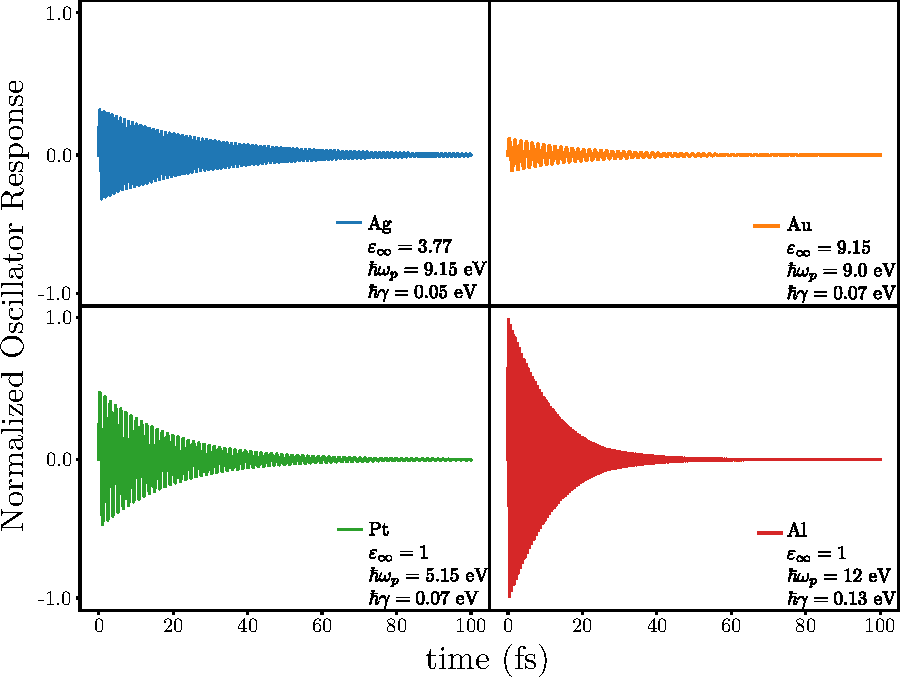
\includegraphics{all_alpha.pdf}
\caption{Normalized, time-dependent response of the (a) silver, (b) gold, (c) platinum, and (d) aluminum dipole plasmon over a span of 100 fs. The maximum amplitude is related to the high-frequency dielectric constant, $\varepsilon_{\infty}$, the oscillation frequency is determined by $\sqrt{\omega_{\textrm{sp}}^2 - \gamma^2/4}$, and the decay rate is $\gamma$, which contains contributions from electron-ion scattering and radiation damping.}
\label{alpha_metals}
\end{centering}
\end{figure}


\section{Multiple Metal Nanoparticles}

The hybridization of dielectric grains was the first major study on plasmon hybridization theory\cite{Lucas1976}. This work showed that when multiple dielectric micro- or nanoparticles are brought close together, they exhibit collective optical properties rather than their individual optical properties. Since then, this concept has been central to the study of plasmonics. There have been numerous hybridization models, from coupled dipole approaches\cite{Schatz2003} to molecular orbital-like approaches\cite{Oubre2004,NordProdan2004}. Many of these studies have inspired the work in this thesis. Previous work has investigated the distance-dependence of collective resonance wavelength and radiation damping\cite{vonPlessen2007} and the impact of environment on MNP coupling strength\cite{Elsayed2008}. Much work has also been done to show the spectroscopic impacts of hybridization\cite{Xu1995,Mischenko1995}. It is thanks to these studies that we now have a rich understanding of and language describing MNP interactions. 

Plasmon hybridization theory matters because it informs real-world applications. MNP dimers have been shown to make effective rulers\cite{Ruler}. Small clusters have also been shown to be effective substrates for surface enhanced raman spectroscopy\cite{SERS}. In Chapter 2, we will discuss how hybridization is a possible measure of energy transfer; similarly, there has been much effort to investigate how a MNP hybridizes with and transfers energy to other MNPs and to its environment\cite{CubeSubstrate,ARAVIND1981,ThakkarLandau}. Plasmon hybridization is at its core an analogy for the transfer of electromagnetic information. Understanding how multiple MNPs interact with one another is central to the work presented in this thesis and to much of the field of plasmonics and its applications.

Who to cite: Lukas, von Plessen, El Sayed, Schatz, others studying plasmon hybridization
\subsection{The Quasistatic Limit}
Bringing two atoms close together causes their atomic orbitals to mix, forming new, hybridized molecular orbitals [citation needed]. These molecular orbitals are the basis of bonds. For instance, the molecular orbitals of $\textrm{H}_2$ formed from two H $s$-orbitals split into a lower energy, bonding orbital and a higher-energy, anti-bonding orbital. Pairs of LSPRs behave similarly. When brought close to each other, they hybridize and produce new normal modes, one lower energy and one higher energy. We have just learned that we can model the response of a LSPR as a harmonic oscillator. By extension, we can treat pairs (or larger collections) of LSPRs as systems of coupled oscillators whose dynamics depend on each other. Dipole LSPRs couple through a pairwise interaction between each dipole and the field produced by each other dipole ($U = -\sum_{j\neq i}\textbf{d}_i\cdot\textbf{E}_j/2$). This interaction is mediated by something called the dipole relay tensor
\begin{equation}
\boldsymbol{\Lambda}_{ij} = \left\{\left(\frac{1}{r_{ij}^3} - \frac{ik}{r_{ij}^2}\right)\left(3\hat{\textbf{n}}_{ij}\hat{\textbf{n}}_{ij} - \textbf{1}\right) - \frac{k^2}{r_{ij}}\left(\hat{\textbf{n}}_{ij}\hat{\textbf{n}}_{ij} - \textbf{1}\right)\right\}\frac{e^{\textrm{i}kr_{ij}}}{\varepsilon_b}
\label{dipole_relay_tensor_full}
\end{equation}
where the $i$th and $j$th dipoles are displaced by $r_{ij}\hat{\textbf{n}}_{ij}$ and $k=\sqrt{\varepsilon_b}\omega/c$. To build intuition about this tensor, we will consider a simple example: two dipoles, separated by $s\hat{\textbf{x}}$, with equal dipole magnitudes and dipole directions perpendicular to the direction of displacement ($\hat{\textbf{y}}$, see Fig. \ref{dimer_stat}). Eq. \ref{dipole_relay_tensor_full} represents the fully retarded dipole relay tensor, i.e., it takes into account that information propagates at the speed of light and takes time to travel from one MNP to the other. However, if the MNPs are much smaller than a wavelength of light such that $ka \ll 1$, we can approximate the speed of light as infinite. This means that information propagates across the MNP aggregate almost instantaneously, or at least faster than the lifetime of any relevant excitations. For example, the lifetime of a typical LSPR, as shown in Fig. \ref{alpha_metals}, is on the order of ten femtoseconds. Meanwhile, light travels across a 10 nm MNP in less than one femtosecond, much faster than a plasmon's lifetime. This is called the quasistatic approximation, and taking all of this into account the dipole relay tensor reduces to
\begin{equation}
\lim_{ka \to 0}\boldsymbol{\Lambda}_ij =  \frac{3\hat{\textbf{n}}_{ij}\hat{\textbf{n}}_{ij} - \textbf{1}}{r_{ij}^3}.
\end{equation}
[As its name suggests, the dipole relay tensor describes how two dipoles communicate with one another. The interaction energy between two dipoles is found by computing the left dot product of one dipole with $\Lambda_{ij}$ and the right dot product of the other dipole with $\Lambda_{ij}$. It can also be shown that $\Lambda_{ij}\cdot\textbf{d}_j = \textbf{E}_j$ where $\textbf{d}_j$ is the dipole moment of the $j$th dipole with electric field $\textbf{E}_j$. Using the previously defined geometry, namely two parallel dipoles $\textbf{d}_i,j = eq\hat{\textbf{y}}$ separated by $s\hat{\textbf{x}}$, we can compute the interaction energy
\begin{equation}
\begin{split}
U &= -\textbf{d}_1\cdot\boldsymbol{\Lambda}_{12}\cdot\textbf{d}_2\\
&= -e^2q^2\hat{\textbf{y}}\cdot\frac{3\hat{\textbf{x}}\hat{\textbf{x}} - \textbf{1}}{s^3}\cdot\hat{\textbf{y}}\\
&= \frac{e^2q^2}{s^3}
\label{quasi_int}
\end{split}
\end{equation}
The interaction energy for a pair of parallel dipoles carries a positive sign, indicating that it is repulsive in nature, and depends on the magnitudes of the dipole moments and the cube of separation distance between them. The same procedure reveals similar dependence but different coefficients for anti-parallel, collinear, and anti-collinear dipole orientations. Those coefficients are indicated in Fig. \ref{dimer_stat}.

\begin{figure}
\begin{centering}
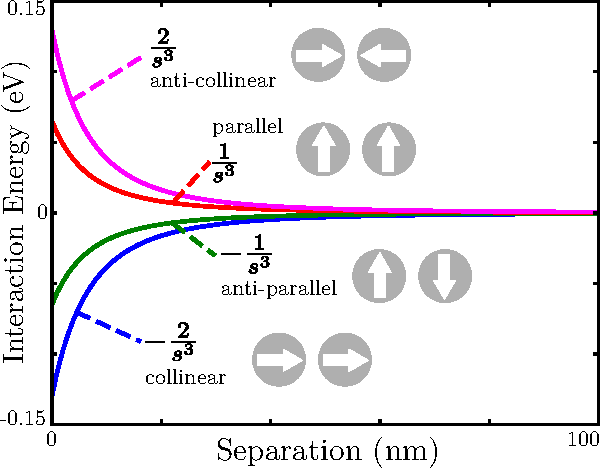
\includegraphics{dimer_stat.pdf}
\caption{Quasistatic interaction energies for (color) collinear, (color) anti-parallel, (color) parallel, and (color) anti-collinear arrangements of dipoles in a dimer of $a=20$ nm silver spheres plotted against increasing seapration distance, from touching to 100 nm apart. Note that with increasing distance, all of the interactions tend towards zero and remain in the same energy-order.}
\label{dimer_stat}
\end{centering}
\end{figure}

In Fig. \ref{dimer_stat} the quasistatic interaction energies are shown as a function of distance for each of the four dipole arrangements. All of the interaction energies fall to zero with increasing $s$, and the energy-ordering of the dipole arrangements is constant. We will soon find that rejecting the quasistatic approximation and demanding that the speed of light be finite breaks this intuition.

\subsection{Retardation Effects}

Plasmon hybridization in the retarded regime has also been well explored. [cite the same papers from your second paper] Going back to Equation \ref{dipole_relay_tensor_full} in full, we can perform the same procedure as above to compute the fully retarded interaction energy between pairs of dipoles. For the parallel arrangement, this becomes
\begin{equation}
U = e^2q^2\left(\frac{1}{s^3}-\frac{\textrm{i}k}{s^2}-\frac{k^2}{s}\right)e^{\textrm{i}ks}.
\label{int_ret}
\end{equation}
The interaction energy now has terms that depend on $k$, and through that, the oscillation frequency $\omega$. We will soon see that this collective frequency, $\omega$, in turn depends on the interaction energy, meaning that this entire problem must be solved iteratively. Also interesting to note is that each term carries a different sign and the entire energy carries a complex exponential, a term that oscillates with changing $s$. So, as a function of increasing separation distance, the individual terms in the interaction energy will change character from attractive to repulsive. Fig. \ref{dimer_ret} shows, for each dipole arrangement, the contributions of each term in the interaction energy and the total interaction energy as a function of separation distance. Unlike the interaction energy in the quasistatic limit, which is made of only one non-oscillating term, the fully retarded interaction energy changes both magnitude and sign as a function of distance.

\begin{figure}
\begin{centering}
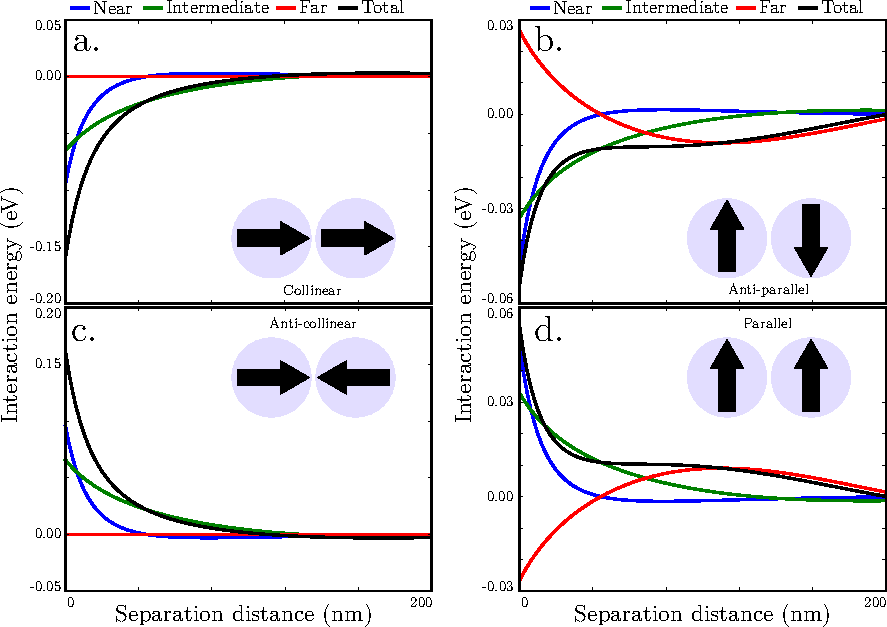
\includegraphics{dimer_ret.pdf}
\caption{Fully retarded interaction energies for (a) collinear, (b) anti-parallel, (c) parallel, and (d) anti-collinear arrangements of dipoles in a dimer of $a=20$ nm silver spheres plotted against increasing separation distance, from touching to 100 nm apart. The fully retarded calculations include the (color) near-, (color) intermediate-, and (color) far-field contributions to the (black) total interaction energy. There are distinct regions of space where each of the terms of the field has the greatest magnitude. Note that with increasing distance, all of the interactions tend towards zero.}
\label{dimer_ret}
\end{centering}
\end{figure}

The insight gained from this exercise is that the ``bonding'' or ``anti-bonding'' character of an arrangement of dipoles actually depends on the separation distance between the dipoles and their collective frequency. Fig. \ref{dimer_ret_tot} compares the total interaction energy for all four arrangments of dipoles, showing that as a function of separation, the spectral ordering of the collective modes changes with separation.

\begin{figure}
\begin{centering}
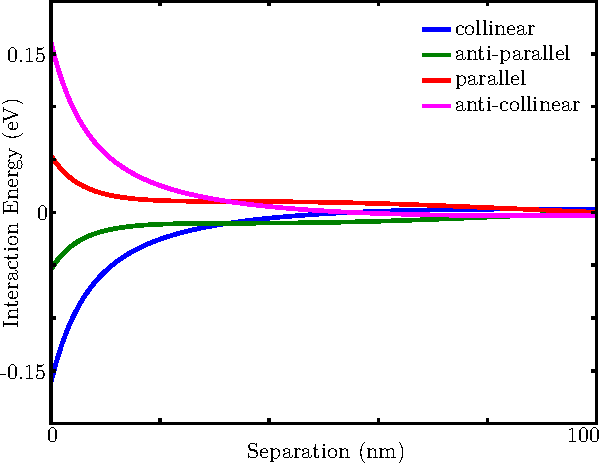
\includegraphics{dimer_ret_total.pdf}
\caption{Fully retarded total interaction energies for (color) collinear, (color) anti-parallel, (color) parallel, and (color) anti-collinear arrangements of dipoles in a dimer of $a=20$ nm silver spheres plotted against increasing seapration distance, from touching to 100 nm apart. Note that with increasing distance, all of the interactions tend towards zero and change energy-order to the oscillatory nature of the electric field.}
\label{dimer_ret_tot}
\end{centering}
\end{figure}

The dipole relay tensor, $\boldsymbol{\Lambda}_{ij}$, informs the basis of the work presented in this thesis, namely the study of the interactions between multiple MNPs. In Chapter 2, we will discuss how we can study the plasmonic spectrum of non-spherical MNPs by modeling them as small clusters of spherical MNPs well within the quasistatic limit. We will further extend this quasistatic model to incorporate mixed-metal systems and to interpret the results of full-wave simulations. In Chapter 3 we learn more about the impact of aggregation scheme and nanocluster size, and how retardation effects and plasmon hybridization play a role in the spectral ordering of collective plasmon modes. Throughout this thesis we will refer back to the dipole relay tensor. It is a concept central to the understanding of the behavior of more than one MNP. Finally, at the very end of this thesis, we will breifly introduce work on predicting the results of photon-assisted electron spectroscopies, a recent experimental collaboration that shows much potential.
\newpage
\section{List of publications}
\begin{enumerate}
\item West, B. A., Molesky, B. P., Montoni, N. P., and Moran, A. M. ``Nonlinear optical signatures of ultraviolet light-induced ring opening in $\alpha$-terpinene.'' {\it New J. Phys.}, {\bf 2013}, {\it 15}, 025007.
\item Quillin, S. C., Cherqui, C., Montoni, N. P., Li, G., Camden, J. P., and Masiello, D. J. ``Imaging plasmon hybridization in metal nanoparticle aggregates with electron energy-loss spectroscopy.'' {\it J. Phys. Chem. C}, {\bf 2016}, {\it 120}, 20852-20859.
\item Griffin, S., Montoni, N. P., Li, G., Straney, P. J., Millstone, J. E., Masiello, D. J., and Camden, J. P. ``Imaging energy transfer in Pt-decorated Au nanoprisms via electron energy-loss spectroscopy.'' {\it J. Phys. Chem. Lett.}, {\bf 2016}, {\it 7}, 3825-3832.
\item Cherqui, C., Wu, Y., Li, G., Quillin, S. C., Busche, J. A., Thakkar, N., West, C. A., Montoni, N. P., Rack, P. D., Camden, J. P., and Masiello, D. J. ``STEM/EELS imaging of magnetic hybridization in symmetric and symmetry-broken plasmon oligomers dimers and all-magnetic Fano interference.'' {\it Nano Lett.}, {\bf 2016}, {\it 16}, 6668-6676. 
\item Thakkar, N., Montoni, N. P., Cherqui, C., Masiello, D. J. ``Plasmonic Landau damping in active environments." {\it Phys. Rev. B}, {\bf 2018}, {\it 97}, 121403.
\item Montoni, N. P., Quillin, S. C., Cherqui, C., Masiello, D. J. ``Tunable spectral ordering of magnetic plasmon resonances in metal nanoclusters.'' {\it In preparation}, 2018.
\item Montoni, N. P., Busche, J. A., Rack, P. D., Duscher, G., and Masiello, D. J. ``Stimulated electron energy-loss spectroscopy.'' {\it In preparation}, 2018.
\end{enumerate}
% ========== Chapter 2
 
\chapter{Imaging Energy Transfer in Pt-decorated Au Nanoprisms via Electron Energy-loss Spectroscopy}

\begin{ch_abstract}
Driven by the desire to understand energy transfer between plasmonic and catalytic metals for applications such as plasmon-mediated catalysis, we examine the spatially resolved electron energy-loss spectra (EELS) of both pure Au nanoprisms and Pt-decorated Au nanoprisms. The EEL spectra and the resulting surface-plasmon mode maps reveal detailed near-field information on the coupling and energy transfer in these systems, thereby elucidating the underlying mechanism of plasmon-driven chemical catalysis in mixed-metal nanostructures. Through a combination of experiment and theory we demonstrate that although the location of the Pt decoration greatly influences the plasmons of the nanoprism, simple spatial proximity is not enough to induce significant energy transfer from the Au to the Pt. What matters more is the spectral overlap between the intrinsic plasmon resonances of the Au nanoprism and Pt decoration, which can be tuned by changing the composition or morphology of either component.
\end{ch_abstract}

Localized surface plasmon resonances (LSPRs), the quantized oscillation of the free electron gas in metal nanoparticles, underlie a variety of applications ranging from surface-enhanced spectroscopy\cite{Nie1997,Schlucker,SERS_1,SERS_femto,COINs} and sensing\cite{PCCP,SpecSense} to solar energy harvesting\cite{OPV,waveguides,SiSolar,RiceCrew}. Plasmons in noble metals commonly occur in the visible part of the spectrum and can focus light to subdiffraction limited spots, thereby converting light energy from the far-field into the near-field. The exceptionally large polarizability of nanoparticles at the resonance frequency of the LSPR results in absorption cross sections that can be more than an order of magnitude larger than the particle’s physical size. There is great interest, therefore, in utilizing this light-harvesting property to drive chemical reactions\cite{aminothiophenol,PtAuRods,PtAuPrisms,Halas2013} or improve solar device efficiency\cite{OPV,SiSolar,Linic}. There is also a growing body of evidence indicating that LSPR excitation can drive otherwise unfavorable reactions such as the conversion of 4-aminothiophenol (4ATP) to 4,4′-dimercaptoazobenzene (DMAB),\cite{aminothiophenol,nitrobenzenethiol,KimKimShin} H$_2$ dissociation on Au\cite{Halas2013}, liquid water splitting\cite{watersplitting,photoanodes,Thimsen}, hydrocarbon conversion\cite{Cronin}, and gas-phase oxidation\cite{LinicSilver}.

Bimetallic systems, composed of catalytic and plasmonic metals, are especially interesting because they provide a potential route to further increase the efficiency of plasmon-driven chemical reactions. However, the plasmon resonances of common catalytic metals, e.g., Pd, Pt, and Rh, occur at energies much higher than those of noble metals and are lossy\cite{Weaver}. Nevertheless, recent studies demonstrate plasmon-enhanced energy transfer is applicable in catalytic chemistry\cite{LinicCharge,LinicDominant,RingeHetero}. Wang et al.\cite{YanSuzuki}, for example, showed that Pd-decorated Au nanorods can catalyze a Suzuki coupling of bromobenzene and m-tolylboronic acid upon plasmon excitation. Zheng et al.\cite{PtAuRods} observed a similar phenomenon where Au nanorods and nanospheres with pendant Pt nanoparticles could catalyze H2 evolution, and they speculated that hot-electron generation via decay of the Au LSPR drives the reaction.

Electron energy-loss spectroscopy (EELS), performed in a monochromated scanning transmission electron microscopy (STEM) instrument, is especially promising for studying energy transfer between plasmonic and catalytic metals because it combines subnanometer spatial resolution with spectral resolution of approximately 100 meV\cite{ARPC}. Recently, for example, Li et al.\cite{CubeSubstrate} illustrated how EELS can spatially map energy transfer from individual plasmonic nanocubes to their semiconductor substrates; Wu et al.\cite{Alloys} explored the plasmonic properties of size-tunable alloy systems; and Ringe et al.\cite{RingeTips} studied Pd-coated Au nano-octopods revealing strong EEL signals at the Pd-coated tips.

While previous work has established the viability of plasmon-assisted chemistry in mono- and bimetallic nanostructures, fundamental studies of plasmon hybridization in well-defined, mixed-metal systems are needed to elucidate the mechanisms underlying these observations. Because of their well-characterized plasmonic properties, in this Letter we investigate bare Au nanoprisms and Au nanoprisms decorated with spherelike, dendritic Pt nanoparticles (Au+Pt) in order to gain an understanding of the coupling between optical and catalytic properties in bimetallic nanostructures\cite{MillstoneSeedless,MillstonePtAu}. STEM/EELS measurements and full-wave numerical EELS simulations are performed on pure Au nanoprisms and Pt-decorated Au nanoprisms, respectively, to understand how unperturbed Au plasmon modes are deformed by the location of the Pt particle. This work provides a nanoscopic view of how the plasmon mode structure of Au nanoprisms changes both spatially and spectrally in the presence of Pt and provides insight into energy transfer between Au and Pt constituents within the mixed-metal system. Using EELS simulations only, we further find that the LSPRs of an Al nanoprism will spectrally overlap with the LSPR of Pt, resulting in coupling stronger than that of the Au+Pt system.

Figures \ref{modes_tip} and \ref{modes_center} display the high-angle annular dark-field (HAADF) images and compare the experimentally acquired EEL maps with EELS simulations for two different Au+Pt geometries: a 209 nm edge length Au nanoprism with a 40 nm diameter Pt particle deposited at the tip (Figure \ref{modes_tip}d) and a 198 nm edge length Au nanoprism with a 40 nm diameter Pt particle deposited at the center of the prism (Figure \ref{modes_center}d). In each case, we compare the data obtained from the decorated particles with data from bare Au nanoprisms of the same size (Figures \ref{modes_tip}a and \ref{modes_center}a) to study the influence of the Pt particle on the plasmon mode structure. The loss energies for the mode maps are selected using the peak maxima of the point EEL spectra when the electron beam is positioned at the tip, edge, corner, and face and on the Pt decoration. These beam positions are selected as representative points of the LSPR modes of the nanoprism and Pt decoration. All experimental nanostructures are supported on a 30 nm thick Si3N4 membrane, and all simulations are performed in vacuum.

\begin{figure}
\begin{centering}
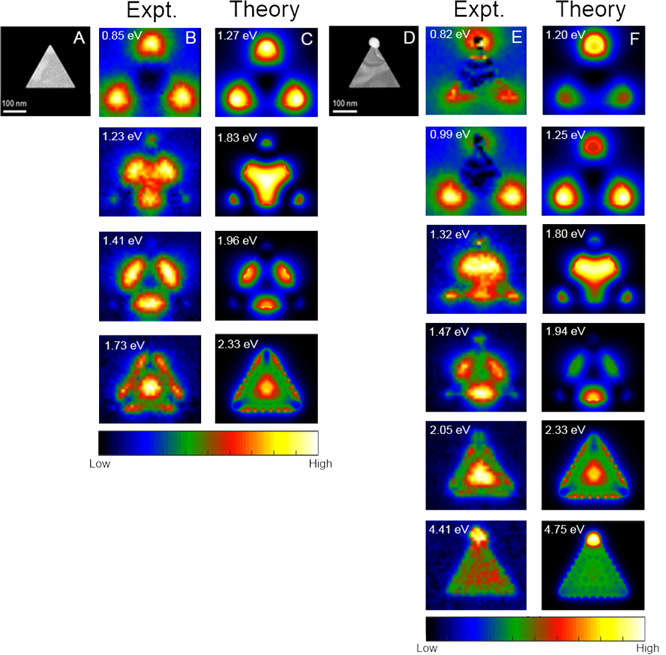
\includegraphics{prisms_mode_maps_tip.png}
\caption{(A-C) Experiments and simulations for a bare Au nanoprism, 209 nm edge length and 10 nm in thickness, supported on a Si3N4 membrane. (A) HAADF; (B) Experimentally measured EEL maps for loss-energies representing corner, edge, and facial plasmon modes; (C) Simulated EEL maps. (D-F) Experiments and simulations for a Au nanoprism, 209 nm edge length and 10 nm in thickness, decorated with a 40 nm diameter Pt nanoparticle supported on a Si3N4 membrane. (D) HAADF; (E) Experimentally measured EEL maps for loss-energies representing corner, edge, facial, and Pt plasmon modes; (F) Simulated EEL maps. Note the splitting of the plasmon modes in the vicinity of the Pt particle (0.85 eV) and the mode mixing induced by the Pt particle at higher loss-energies. Experimental and calculated loss- energies for each mode differ as simulations are calculated in vacuum.}
\label{modes_tip}
\end{centering}
\end{figure}

\begin{figure}
\begin{centering}
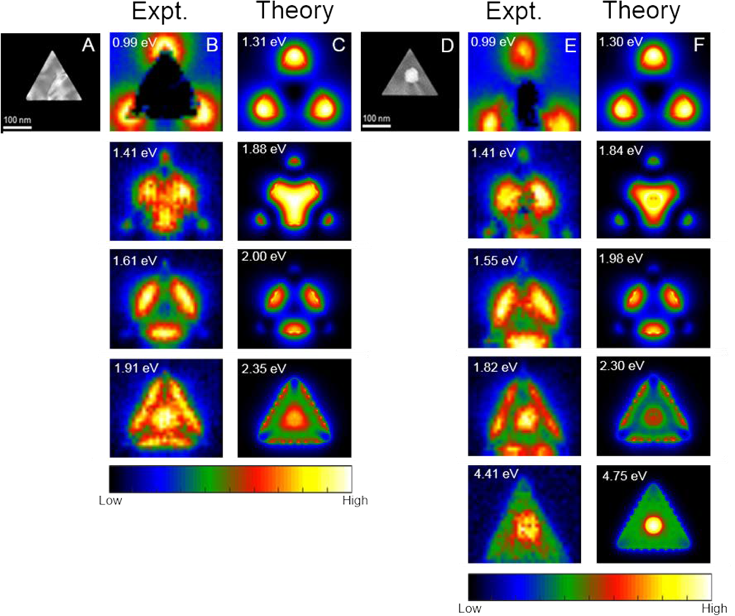
\includegraphics{prisms_mode_maps_center.png}
\caption{(A-C) Experiments and simulations for a bare Au nanoprism, 195 nm edge length and 10 nm in thickness, supported on a Si3N4 membrane. (A) HAADF; (B) Experimentally measure EEL maps for loss-energies representing corner, edge, and facial plasmon modes; (C) Simulated EEL maps. (D-F) Experiments and simulations for a Au nanoprism, 198 nm edge length and 10 nm in thickness, decorated with a 40 nm diameter Pt nanoparticle supported on a Si3N4 membrane. (D) HAADF; (E) Experimentally measure EEL maps for loss-energies representing corner, edge, facial, and Pt plasmon modes; (F) Simulated EEL maps. Note that the low-energy mode structure is conserved between the decorated and undecorated particles due to the three-fold symmetry when Pt is at the center of the prism. Experimental and calculated loss energies for each mode differ as simulations are calculated in vacuum.}
\label{modes_center}
\end{centering}
\end{figure}

Figures \ref{modes_tip}b and \ref{modes_center}b show that the plasmon modes of the bare prisms evolve from dipoles localized to the corners, through those on the edges, and finally into multipolar modes as a function of increasing energy, which is in excellent agreement with previous EELS studies of plasmonic nanoprisms\cite{ColliexMapping,ColliexEELS}. Interestingly, a comparison of the mode maps resulting from decorated and undecorated prisms (Figure \ref{modes_tip}b,e) shows minimal changes to the mode structure upon addition of the Pt particle. The most notable difference is seen in the splitting of the dipolar mode of the bare Au nanoprism, where the presence of the Pt particle breaks the degeneracy of the dipole mode (vide infra) (Figure \ref{modes_tip}b,e). Figure \ref{modes_center}b,e illustrates that the structure of the higher-energy modes is not strongly dependent on the Pt particle location, as the EEL maps in Figures \ref{modes_tip}b,e and \ref{modes_center}b,e are similar. Lastly, we are able to experimentally map the LSPR of the Pt decoration at a higher energy than the modes of the nanoprism (Figures \ref{modes_tip}e and \ref{modes_center}e).

Boundary element method calculations\cite{Hohenester2012,Hohenester2014} (Figures \ref{modes_tip}c,f and \ref{modes_center}c,f) capture the complex mode structure of these mixed-metal systems and agree well with the experimental measurements (Figures \ref{modes_tip}b,e and \ref{modes_center}b,e). While there are quantitative differences in specific plasmon resonance energies between simulation and experiment due to substrate effects, we can leverage the qualitative agreement in the equivalent mode identity to explore the perturbative effects of Pt on the well-understood LSPR modes\cite{HohenesterDisk} of Au nanoprisms with plasmon hybridization theory. Previous work\cite{Nanodecahedra,Decahedra} has shown that a basis set composed of corner-localized dipoles is sufficient to interpret the low-energy plasmon mode structure of the Au+Pt system. Therefore, we create a model composed of dipoles located on the corners of a triangular prism\cite{Quillin,Zohar}. Each corner is represented by a disk with two in-plane, orthogonal, dipole plasmons. These single-disk dipoles can be rigorously mapped onto a set of mechanical oscillators and mutually hybridized by diagonalizing the Hamiltonian\cite{Cherqui2014}
\begin{equation}
H = \frac{1}{2}\sum_{i}\hbar\omega_{\textrm{sp}^i}[\textbf{P}_i^2 + \textbf{Q}_i^2] - \frac{1}{2}\sum_{i \neq j}\hbar(\omega_{\textrm{sp}}^i\omega_{\textrm{sp}}^j)^{1/2}g_{ij}(r_{ij})[3(\textbf{Q}_i\cdot\hat{\textbf{n}}_{ij}\hat{\textbf{n}}_{ij}\cdot\textbf{Q}_j)-\textbf{Q}_i\cdot\textbf{Q}_j],
\label{prism_hammy}
\end{equation}
with distance-dependent coupling constants $g_{ij}(r_{ij}) = 3/[r_{ij}^3(\varepsilon_{\infty} + 2)]$ where $i$ and $j$ ($i, j = 1–6$) indicate the identity of each plasmon (location and orientation); $\textbf{Q}_i$ is the coordinate of the $i$th oscillator with conjugate momentum $\textbf{P}_i$; $\omega_{\textrm{sp}}^i$ is its surface plasmon resonance frequency; $r_{ij}$ are the dimensionless distances between the $i$th and $j$th disks relative to their diameters; and $\hat{\textbf{n}}_{ij}$ is the corresponding unit vector connecting them.
In analogy to the mixing of carbon p-orbitals in benzene, the mixing of these six single-disk modes result in six hybridized modes: the lowest-energy mode having no nodes; the second lowest being two degenerate, single-node modes (dipole modes); the third lowest being two degenerate, double-node modes; and the highest-energy mode having three nodes. To produce a quantitative fit to the experimental and simulated data, we choose the resonance frequencies of the disk plasmons so that the resulting dipole plasmon resonance of the Au prism produces the experimentally measured resonance energy (∼1.00 eV).

With this simple model in hand, we are now able to explore the perturbing effects of a Pt particle. Simulation using experimentally derived dielectric data\cite{Weaver} predicts the plasmon resonance of the Pt particle to be near 5.00 eV, which is at a significantly higher energy than the LSPR modes of the Au nanoprism. We introduce the Pt particle to the system as a disk with two degenerate, in-plane, orthogonal dipoles with resonance energies of 5.00 eV, as dictated by experiment on single Pt particles. The plasmon resonances of the collective system are explored with the same hybridization method as before.

Figure 3 displays the hybridization model describing the interaction between the Au nanoprism dipole modes and the Pt dipole modes together with corresponding experimental EEL maps that illustrate the effect of the Pt on the Au nanoprism. Depositing the Pt particle at the center of the nanoprism gives the system 3-fold symmetry and, in turn, does not significantly perturb the LSPR modes of the nanoprism. The mode mixing does cause a small, equal net lowering of the prism-localized collective dipole modes and a small, equal net raising of the Pt-localized collective dipole modes. As the Pt particle is moved toward a corner, however, the system’s dipole modes begin to split. When the prism and the Pt-localized dipole modes are oriented in the same direction, they couple more strongly than when the dipoles are oriented antiparallel; therefore, the former is lower in energy, as expected\cite{Quillin}. The model further shows that this splitting is maximal when the Pt particle is as close to the corner as possible, which is consistent with experimental results.

\begin{figure}
\begin{centering}
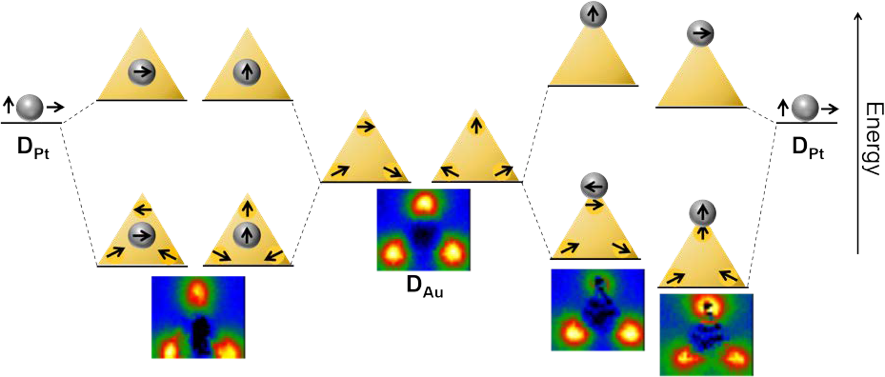
\includegraphics{prisms_theory.png}
\caption{Dipole oscillator model of the mode mixing between the Au prism dipoles (DAu) and the Pt sphere dipoles (DPt). The anti-bonding Pt-centered modes are blue-shifted far from the prism modes upon mixing; whereas, the bonding modes remain centered on the nanoprism and depend much more noticeably upon the placement of the Pt particle. Placing the Pt particle in the center of the Au prism (left) causes a net lowering of the dipole modes but no splitting. The lack of splitting is observed experimentally in the 0.99 eV mode map. Placement of the Pt particle at the tip (right) induces splitting between the formerly degenerate dipolar prism modes, as observed in the experimentally derived mode maps at 0.99 eV and 0.82 eV loss-energies.}
\label{mo_diagram}
\end{centering}
\end{figure}

Figure 4a compares the simulated EEL spectra of a 209 nm pure Au nanoprism (black), a 209 nm Au+Pt nanoprism (red) where the 40 nm diameter Pt decoration is at the tip of the nanoprism, and an aloof EEL spectrum of a 40 nm diameter Pt sphere (purple). The Au nanoprism is plasmonically active at energies between 0.90 and 2.40 eV, whereas the Pt sphere is active at a much higher energy (∼5.00 eV). Because of the spectral mismatch in plasmon resonance energies of Au and Pt, these metals are not expected to significantly hybridize and resonance energy transfer is unfavorable. The Pt decoration, therefore, simply acts as part of the dielectric environment, and the plasmons of the prism couple to their images in the Pt particle and vice versa. This image effect is identical for all of the Au and Pt dipole plasmons in the center-decorated system. However, in the tip-decorated system, the nanoprism dipole that is aligned with the Pt dipole couples more strongly to its image than the other orthogonal dipole and is shifted to lower energy.

\begin{figure}
\begin{centering}
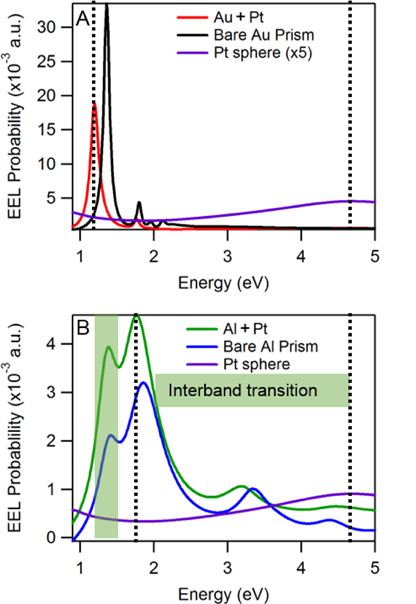
\includegraphics{prisms_EELS_simulation.png}
\caption{Comparison of the calculated EEL spectra at the tip of (A) a 209 nm pure Au nanoprism (black trace), a 209 nm Au+Pt nanoprism (red trace), and a 40 nm diameter Pt sphere (purple trace); (B) a 209 nm bare Al nanoprism (blue trace), a 209 nm Al+Pt nanoprism (green trace), and a 40 nm diameter Pt sphere (purple trace). The interband transition of the Al is centered at 1.40 eV (green box). For each decorated system, the Pt particle is 40 nm in diameter and located at the tip of the nanoprism. Note the slight shifting (~0.15 eV) and broader line- width (FWHM increases by 0.30 eV) in the Al+Pt at ~3.20 eV. This broadening indicates LSPR hybridization between the two metals; whereas, in the Au+Pt system there is a shift of 0.03 eV and a small change in the line-width (FWHM increases by 0.005 eV) at ~1.80 eV. The black dotted lines at 1.20, 1.75, and 4.75 eV correspond to the LSPR of Au+Pt, Al+Pt, and Pt, respectively.}
\label{prisms_EELS_sim}
\end{centering}
\end{figure}

The framework presented here, while showing that the Au and Pt plasmons remain mostly uncoupled, does offer insight into the construction of systems with highly coupled plasmon modes for plasmon-mediated catalysis. Consequently, we study Al prisms\cite{Aluminum,AluminumHydrogen} decorated with Pt because the Al plasmons lie at energies higher than those of Au\cite{NordHalAluminum}. Figure 4b compares simulated EEL spectra for a 209 nm Al nanoprism (blue), a 209 nm Al+Pt nanoprism (green) with a 40 nm Pt tip decoration, and a 40 nm diameter Pt sphere (purple). The spectrum of the 3.20 eV peak in the Al+Pt system is broadened by 0.31 eV, determined from the full width at half-maximum (fwhm), with respect to the higher-energy Al prism-localized LSPR modes (∼3.20 eV), suggesting stronger hybridization with the Pt dipole plasmons than in the Au+Pt system. Both Pt and Al have low-energy interband transitions (0.90 and 1.40 eV, respectively) that are not expected to hybridize because of their poor spectral overlap\cite{Segall}.

To further explore the properties of Al coupled with Pt, Figures 5 and 6 compare the magnitude of the electron-beam-induced electric near-fields of the Al+Pt and Au+Pt systems at three loss-energies: 1.20, 1.75, and 4.75 eV, as indicated in Figure 4 (dotted, vertical lines). Qualitatively similar electric near-fields would arise in response to linearly polarized plane-wave excitation because of the common polarization it shares with the field of the electron at the indicated beam position (x). The field maps reveal that at the energy of the prism-localized dipole mode (Figure 5a,b) and the energy of the Pt-localized dipole mode (Figure 5c,d), the fields around the Pt particles are similar in magnitude. This is reinforced in Figure 5e,f, which present the electric field magnitudes computed along lines (white) bisecting the Pt particle and clearly show electric fields of similar magnitudes for both systems.

\begin{figure}
\begin{centering}
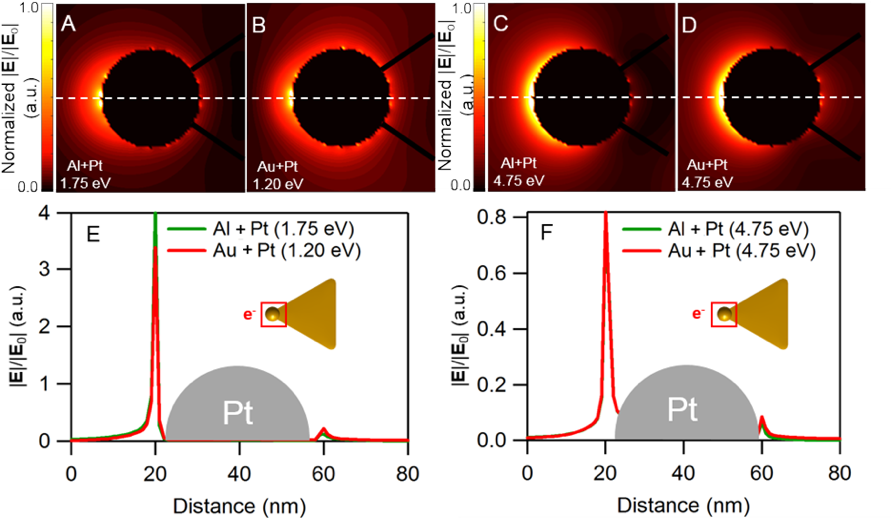
\includegraphics{prisms_field_calculations.png}
\caption{Electric field maps, resulting from electron beam excitation (e-), computed in the plane bisecting the Pt particle and above the prism at the resonance frequencies of the prism dipole plasmons for Al+Pt (A, 1.75 eV) and Au+Pt (B, 1.20 eV). Electric field maps are computed for the same systems, Al+Pt (C) and Au+Pt (D), at the Pt dipole plasmon. Note that the fields become more diffuse around the tip at the Pt resonance frequency (4.75 eV). The fields along the white dotted line are plotted for the prism dipole resonance of Al+Pt and Au+Pt (E, green and red traces, respectively), and for the Pt dipole resonance in Al+Pt and Au+Pt (F, green and red traces, respectively). The gray shapes mark the positon of the sphere. Note that the fields are much larger at the low-energy, hybridized dipoles, but for both systems the fields are comparable in magnitude at similar energies.}
\label{field_top}
\end{centering}
\end{figure}

\begin{figure}
\begin{centering}
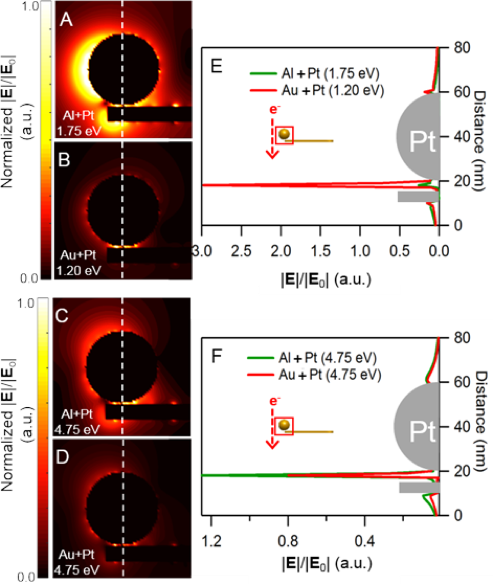
\includegraphics{prisms_fields_2.png}
\caption{Electric field maps, resulting from electron beam excitation (e-), computed in the plane bisecting both the Pt particle and the prism at the resonance frequencies of the dipole plasmons for Al+Pt (A, 1.75 eV) and Au+Pt (B, 1.20 eV) and the dipole plasmon of the Pt (4.75 eV) particle in Al+Pt (C) and Au+Pt (D). Note that the fields in the junction consistently drown out the fields around the particle, except at the dipole of the Al+Pt.
Additionally, along the white dotted line, the fields are plotted for the dipole resonance of Al+Pt and Au+Pt (E, green and red traces, respectively), and for the dipole resonance of the Pt in Al+Pt and Au+Pt (F, green and red traces, respectively). The gray shapes mark the positions of the prism and sphere. Interestingly, the low-energy dipole mode of Au+Pt has a large field in the junction, likely due to Au being a good plasmonic antenna, but the junction field is higher in Al+Pt at the dipole resonance of the Pt. This may be a signature of energy transfer in Al+Pt at these energies.}
\label{field_side}
\end{centering}
\end{figure}

Turning to the field magnitude in the junction at the energy of the prism-localized dipoles (Figure 6a,b), we see that the field is much larger in the Au+Pt junction than in the Al+Pt junction. This means that the junction field in the Au+Pt systems is dominated by the response of the Au nanoprism. Conversely, at the energy of the Pt-localized dipole (Figure 6c,d), the junction field in the Al+Pt system is much larger than that of Au+Pt. These observations are again reinforced by the electric field magnitudes presented in Figure 6e,f, which are computed along lines (white) running through the junction. Taken together, Figures 4–6 indicate a relationship between EEL probability and the strength of the near electric fields surrounding the mixed-metal systems observed in this Letter. These junction fields show that the high-energy modes of the nanoprism are more effectively coupled to the Pt dipole plasmon in Al+Pt than in Au+Pt; therefore, a greater capacity for plasmon-mediated chemical catalysis is predicted in the Al+Pt system. Utilizing the electric near-field simulations and data obtained through experiment and calculations, we show that these plasmonic-catalytic metal systems should drive plasmon-assisted reactions.

This work shows through electrodynamics simulations and experimental EELS the extent to which Au nanoprisms decorated with Pt deposits can transfer energy. EELS demonstrates that Pt changes the mode structure of the Au nanoprism, especially depending on the location of the Pt. Even though we show weak coupling between Au and Pt, we determine stronger coupling can be observed in systems where the LSPRs spectrally overlap. In a system such as Al+Pt, the LSPRs of Al and Pt exhibit more spectral overlap because both metals support LSPRs in the ultraviolet regime.

\section{Methods}

In a typical synthesis, fully described in the Supporting Information, reduction of H2PtCl6 on the surface of AUT (11-amino-1-undecanethiol hydrochloride)-conjugated nanoprisms resulted in the growth of approximately 1–3 Pt nanoparticles (average diameter of 30 ± 5 nm) per Au nanoprism substrate. Using high-resolution transmission electron microscopy (HRTEM), it was found that the Pt nanoparticles had a dendritic morphology (SI Figure 3). Interestingly, nucleation of the Pt nanoparticles occurred predominantly on the edges and vertices of the Au nanoprisms, likely due to the higher concentration of defects in the self-assembled monolayer at these sites\cite{salvarezza}.
Post-synthesis, Au nanoprisms and Pt-decorated Au nanoprisms were sonicated for 5 min and 2.5 μL of each NP solution was drop-cast onto two separate (S)TEM compatible Si3N4 substrates with 30 nm thick membrane acquired from SPI Supplies. These samples were covered to eliminate contamination and left to air-dry for 3 h prior to EELS acquisition. EEL spectra were acquired in a monochromated Carl Zeiss Libra 200MC (S)TEM operated with an accelerating voltage of 200 kV. Each spectrum acquisition was executed with a collection semiangle of 12 mrad, a convergence semiangle of 9 mrad, and a dispersion of 29 meV per channel. Energy resolution, defined as the full width at half-maximum of the zero-loss peak, for each acquisition is 150 meV with the electron beam probing only the Si3N4 membrane. For each nanoprism, EEL spectrum images responsible for producing LSPR mode maps were collected by defining a region of interest (ROI) around the particle with dimensions 34 × 29 pixels, where 1 pixel is ∼3.3 × 3.3 nm2.
Experimentally obtained EELS mode maps are analyzed using Gatan Digital Micrograph software. Experimental EEL LSPR mode maps (Figures 1b,e and 2b,e) are generated by removing the background using the reflected-tail model and normalized to the zero-loss peak. LSPR mode maps were prepared by plotting spectral intensities from energy slices selected from peak maxima of the single-point spectra from the top corner, edge, bottom corner, face, and center of the Pt decoration to fully represent the LSPR modes of the bare Au nanoprism and the Pt-decorated Au nanoprism system.
For simulations, we applied the Metal Nanoparticle Boundary Element Method (MNPBEM) software.(37) MNPBEM represents nanoparticles as surfaces and discretizes each particle into a chosen number of surface elements. Maxwell’s equations are solved at each of these so-called boundary elements in order to calculate the nanoparticle’s optical properties. EELS simulations were performed on Au and Al nanoprisms with edge lengths of 195 and 209 nm and Au+Pt and Al+Pt nanoprism systems with prism edge lengths of 198 and 209 nm and decorated with Pt spheres of diameter 40 nm at the center and tip, respectively. Each system was simulated with no substrate. These simulations used tabulated dielectric data from Johnson and Christy\cite{JC} and Rakic et al.\cite{Rakic} Spectra were acquired at beam positions located at all three corners and edges of each system. Additionally, EEL maps were generated at each of the relevant energy windows. Finally, MNPBEM was used to generate maps of the electric field magnitude around the systems using the electron beam as a source.

% ========== Chapter 3
 
\chapter{Tunable Spectral Ordering of Magnetic Plasmon Resonances in Metal Nanoclusters}
 
\begin{ch_abstract}
Experimental characterization of the optical and magnetic properties of noble metal nanoclusters has exposed a size regime in between single-ring and extended two-dimensional nanocluster networks where the behavior of magnetic plasmon resonances is not well understood. In this intermediate size regime, individual electric dipole plasmons on each nanoparticle within the cluster can hybridize into delocalized magnetic modes that couple to either the electric or magnetic field of light with seemingly arbitrary energy ordering. Here, using a coupled-dipole model that includes fully-retarded interactions between electric dipole plasmons, we show that magnetic plasmon resonance energies can be controllably tuned and even made to cross as a function of nanocluster size. Experimental confirmation of this prediction is challenging because optical selection rules dictate the simultaneous excitation of many spectrally-overlapping magnetic plasmon modes. However, based on analytic modeling and numerical simulation, we show that angle-resolved cathodoluminescence offers an approach to cleanly isolate these magnetic modes and observe the size-dependence of their spectrum. Not only does our work clarify the rich optical and magnetic behavior of noble metal nanoclusters in the intermediate-size regime, but it also suggests strategies to design negative-index plasmonic metamaterials with multiple tunable resonances in the visible spectrum.
\end{ch_abstract}

Plasmon oligomers, or metamolecules, are clusters of noble metal nanoparticles (MNPs) that exhibit anomalously strong magnetic character even though their individual nanoparticle building blocks do not. Known as magnetic plasmons, the collective cyclic oscillation of conduction-band electrons within each cluster has been shown to couple to and enhance the magnetic field of light and to hybridize with other clusters analogously to electric plasmons in individual MNPs \cite{Zhang2006,Zhang2007,NordHal2011,NordHal2012,Cherqui2014,Cherqui2016,Engheta2017}. Since their discovery in 2004 \cite{Shalaev2004}, such magnetic plasmon resonances have been the focus of a body of applied and fundamental research from negative index metamaterials\cite{Alu2006,Alu2008} to quantum tunneling \cite{Dionne2016} and Fano interferences \cite{Dionne2011,Liu2011,Cherqui2016}. The magnetic properties of single oligomers, i.e., those clusters composed of only one ring of MNPs, are now well understood based upon quasistatic modeling, numerical simulation, and optical and electron-beam characterization \cite{Prodan2003,Nord2006,Dionne2011,Dionne2016,Capolino2017}. Infinitely extended two-dimensional networks of oligomers are also well understood theoretically \cite{Schatz2003,Weick2013}. However, recently, a disconnect between these extremes and methods has been discovered \cite{Cherqui2014,Engheta2017}, revealing a lack of understanding of how oligomer assemblies behave in the so-called intermediate size regime \cite{NordHal2011,NordHal2012,Cherqui2014,Qian2015,Cherqui2016,Engheta2017,Fakhraai2018,Scherer2018}.




Central to this disconnect is the question of when and how retardation effects matter. For example, in the case of the two oligomer cluster, the quasistatic approximation deviates from full-wave numerical electrodynamics simulations in that it predicts a different energy-ordering of the two magnetic plasmon resonances \cite{Cherqui2014}. It is well known that retardation effects can affect the electric plasmon energetics in single MNPs \cite{Gu2010}, dimers \cite{Oubre2004,vonPlessen2007}, and infinite chains and arrays \cite{Lucas1976,ARAVIND1981,Kottman2001,Schatz2003,NordHal2003,NordProdan2004,Rechbacher2003,Schatz2003,Royer2005,Abajo2008,Gomez2009,Chumanov2010,Pinchuk2016}. However, to date, no theoretical analysis has been reported on the role of retardation in the description of magnetic plasmon resonances, which are an intrinsically relativistic phenomenon. It is the purpose of this paper to show that the incorporation of retardation corrects the aforementioned disagreement between model and simulation which is pronounced in the intermediate-size regime, and further highlights the ability to tune the magnetic plasmon spectrum by changing the oligomer size. The latter observation is particularly important because it enables manipulation of the system's effective permittivity and permeability, thereby facilitating the design of future tunable optical metamaterials.



In the following, we present a coupled-dipole model to demonstrate the size-dependent evolution of the magnetic plasmons in intermediate-size $N$-ring oligomers, called $N$-mers, by including the effects of retardation in the mutual interaction of their underlying electric dipole plasmon resonances. Interestingly, as a function of size, we find that magnetic plasmon resonances switch their ordering in analogy to the way that electric plasmons in hybridized nanoparticles \cite{vonPlessen2007} and the giant electric and magnetic dipole plasmons of raspberry-like metamolecules \cite{Fakhraai2018} switch order. We further investigate the distinct radiative properties of these magnetic plasmons by computing the angle-resolved cathodoluminescence (CL) spectrum \cite{Hohenester2012,Hohenester2014,Coenen2011,CoPol2011,Polman2014}. CL is ideal over light scattering because the selection rules of the electron probe allow for the preferential excitation of specific magnetic responses, in distinction from light scattering where many broad higher-order electric responses are also excited. Building from the intuition gained, we finally analyze the size-dependent evolution of intermediate-size plasmonic nanoclusters similar to those characterized recently in Ref. \cite{Engheta2017}. We find that the spectral ordering depends not only on aggregate size but also upon morphology, offering a second handle to modify the spectrum. Such understanding may someday lead to advances in superlensing and electromagnetic cloaking at optical frequencies, as these applications benefit directly from the tunability of the system's electric and magnetic response \cite{Pendry03,Fang2005,Cai2007,Pinchuk07,Shalaev2008,Valentine2008,Ferrari09,Tian2018}.







\section{Model Theory}
%%%%%%%%%%%%%%%%%%%%%%%%%%%%%%%%%%%%%%%%%%%%%%%%%%%%%%%%%%%%%%%%%%%%%%%
\begin{figure}
\begin{centering}
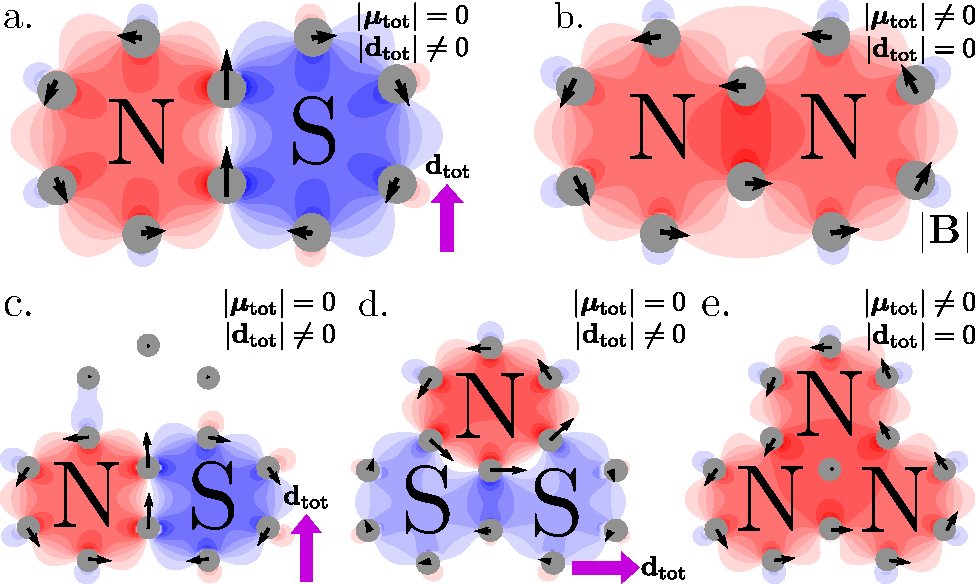
\includegraphics{fig1.pdf}
\caption{Signed magnetic field magnitude of the 2-mer's (a,b) and 3-mer's (c,d,e) magnetic plasmon resonances. Each system supports a number of closed-loop magnetic plasmons equal to the number of rings ($N$) in the oligomer. Magnetic plasmons that have a net electric dipole moment (a,c,d) show a node in their magnetic field and have no net magnetic dipole moment. Oppositely, the nodeless magnetic modes (b,e) possess a net magnetic dipole moment that interacts with the magnetic field of light.}
\label{field_plots}
\end{centering}
\end{figure}
%%%%%%%%%%%%%%%%%%%%%%%%%%%%%%%%%%%%%%%%%%%%%%%%%%%%%%%%%%%%%%%%%%%%%%%
Fig. \ref{field_plots} displays two model oligomer systems, the 2-mer and 3-mer, comprising $n=10$ and $n=13$ silver nanospheres in analogy to the molecules naphthalene and phenalene. The electric plasmons of each MNP can be mapped onto a set of proxy harmonic oscillators as described in Ref. \cite{Cherqui2014,ARPC}. This approach forms the basis for modeling the collective magnetic plasmon responses described herein. In the limit where each nanoparticle, here restricted to a spherical geometry of radius $a$, possesses only an electric dipole plasmon resonance, the hybridized plasmon modes of the oligomer are the solutions of the equations of motion
\begin{equation}
\ddot{\textbf{q}}_i +\omega_{\textrm{sp}}^2\textbf{q}_i = \frac{e}{m_{\textrm{sp}}}\sum_{j\neq i}\textbf{E}_j(\textbf{r}_i),
\label{equation_of_motion}
\end{equation}
where $\omega_{\textrm{sp}}=\sqrt{\omega_{p}^2/(\varepsilon_\infty+2\varepsilon_b)-(\gamma/2)^2}$ is the complex Mie resonance frequency and $m_{\textrm{sp}} = e^2/\alpha_{\textrm{sp}}\omega_{\textrm{sp}}^2$ is the plasmon's effective mass defined in terms of the polarizability $\alpha_{\textrm{sp}} = 3a^3/(\varepsilon_{\infty} + 2\varepsilon_b)$ \cite{Cherqui2014}. Here, $\omega_p$ is the metal's bulk plasma frequency, $\varepsilon_{\infty}$ and $\varepsilon_b$ are the high-frequency and background dielectric functions, and $\gamma$ is well approximated by the sum of the Drude electron-ion scattering and radiation damping rates. While these frictional forces are not explicitly included as velocity-dependent terms in the equations of motion, friction does contribute to the red-shift and linewidth broadening of the Mie resonance with increasing MNP size. The electric dipole moment $\textbf{d}_i = e\textbf{q}_i$ of each plasmon oscillator is restricted to lie in the plane of the oligomer (taken to be the $x-y$ plane) at position $\textbf{r}_i$, and $\textbf{E}_j(\textbf{r}_i)$ is the fully retarded electric field of the $j$th dipole evaluated at the position of the $i$th dipole. The electric field is defined by $\textbf{E}_j(\textbf{r}_i) = \boldsymbol{\Lambda}_{ij}\cdot\textbf{d}_j= \left\{\left(3\hat{\textbf{n}}_{ij}\hat{\textbf{n}}_{ij} - \textbf{1}_{ij}\right)\left({1}/{r_{ij}^3} - {ik}/{r_{ij}^2}\right) - \left(\hat{\textbf{n}}_{ij}\hat{\textbf{n}}_{ij} - \textbf{1}_{ij}\right)k^2/r_{ij}\right\}e^{ikr_{ij}}\cdot\textbf{d}_j/\varepsilon_b,$ where $\hat{\textbf{n}}_{ij}$ is the unit vector connecting two dipoles separated by distance $r_{ij}=|{\bf r}_i-{\bf r}_j|$ and $k=\sqrt{\varepsilon_b}\omega/c.$ The field is decomposed into three parts---the near- ($r_{ij}^{-3}$), intermediate- ($r_{ij}^{-2}$), and far-field ($r_{ij}^{-1}$)---which together include all dipolar retardation effects \cite{Purcell1973}. Interestingly, the latter term carries the opposite sign of the former two. As will be shown in the following, it is because of both the relative magnitude and sign of these terms as well as the oscillatory behavior of $e^{ikr_{ij}}$ that the interactions can change character and switch from energy-lowering to energy-raising. Since magnetic plasmons only involve the hybridization of $(x,y)$-oriented electric dipole plasmons that are orthogonal to the $z$-direction, only those $2n$ (of the $3n$) electric dipole plasmons in the $x-y$ plane are explicitly accounted for in Eq. (\ref{equation_of_motion}).



As described in the Methods Section, there are as many hybridized modes of each $N$-mer as there are electric dipole plasmons. Of these hybrid modes, some are electric and some are magnetic in character, with $N$ magnetic plasmon resonances for each $N$-mer studied here. Fig. \ref{field_plots} shows the magnetic plasmon modes of the 2-mer and 3-mer overlaid with their associated signed magnetic field magnitude. Each mode is named for its particular magnetic field distribution after the poles of a magnet, either all-North (aN) or North-South (NS). The top right-hand corner of each panel indicates the net electric or magnetic dipole moment magnitude. The black arrows denote the electric dipole plasmons on each MNP within each magnetic mode, while the magenta arrow indicates the mode's net electric dipole moment. In planar geometries, the magnetic dipole moments are always perpendicular to the in-plane electric dipole moments. As a result, they scatter light with different directionality as will be discussed.




\section{Spectral Ordering of Magnetic Plasmon Modes in Intermediate-Size $N$-mers}
To determine the impact of incorporating retardation effects, it is first useful to consider the quasistatic limit. Here individual nanoparticle plasmon resonance frequencies ($\omega_{sp}$) are size-independent and the coupling strength depends only upon the scale $s_{ij} = r_{ij}/a$ and not upon the overall oligomer size. That is, if this ratio $s_{ij}$ of interparticle distance $r_{ij}$ to nanoparticle radius $a$ remains constant, the collective resonance frequencies do not change as the nanoparticles increase in size. This is evident by considering the $ka\ll 1$ limit of the interaction on the right-hand side of Eq. (\ref{equation_of_motion}),
\begin{equation}
\begin{aligned}
\lim_{ka \to 0}\frac{e}{m_{\textrm{sp}}}\textbf{E}_j(\textbf{r}_i) &= \frac{e^2}{m_{\textrm{sp}}}\boldsymbol{\Lambda}_{ij}\cdot{\bf q}_j\\ 
&= \frac{\omega_{\textrm{sp}}^2}{\varepsilon_b}\alpha_{\textrm{sp}}\frac{3\hat{\textbf{n}}_{ij}\hat{\textbf{n}}_{ij} - \textbf{1}_{ij}}{r_{ij}^3} \cdot \textbf{q}_j \\
&= \frac{\omega_{\textrm{sp}}^2}{\varepsilon_b} \left(\frac{3}{\varepsilon_{\infty}+2\varepsilon_b}\right)\frac{3\hat{\textbf{n}}_{ij}\hat{\textbf{n}}_{ij} - \textbf{1}_{ij}}{s_{ij}^3} \cdot \textbf{q}_j.
\end{aligned}
\label{quasistatic_coupling}
\end{equation}
Retardation effects, however, remove this invariance and introduce radius-dependence into both the Mie frequency and the electric field. Consequently, in the following, we choose the individual MNP radius $a$ as the independent variable. To define the oligomer geometry, we fix the nearest-neighbor distance to $3a,$ such that the distance between each MNP remains a fixed multiple of $a$ for any value of $a.$

%^ 3$a$ to investigate the effects of retardation upon the magnetic plasmon spectrum in intermediate-size $N$-mers.



%where $m_{\textrm{sp}}$ and $\alpha_{\textrm{sp}}$ are rewritten in terms of fundamental parameters for silver, i.e., $\varepsilon_{\infty} = 3.77$, $\hbar\gamma = 0.05$ eV, and $\hbar\omega_{p} = 9.1$ eV. 




%%%%%%%%%%%%%%%%%%%%%%%%%%%%%%%%%%%%%%%%%%%%%%%%%%%%%%%%%%%%%%%
\begin{figure}
\begin{centering}
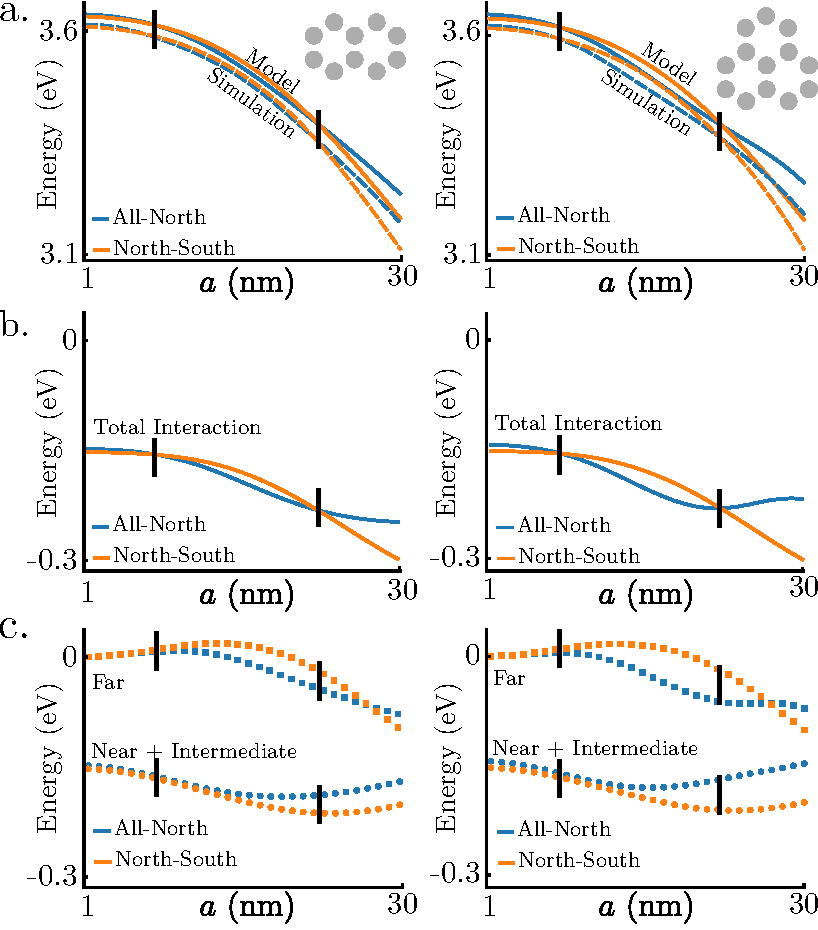
\includegraphics{fig2.pdf}
\caption{(a) Magnetic plasmon resonance energies and (b,c) electric dipole plasmon interaction energies of the 2-mer and 3-mer. For MNP radii $a\lesssim7$ nm, the magnetic modes are ordered as predicted by quasistatic theory, with the NS mode (orange) lower in energy than the aN mode (blue). This implies that for small oligomers, the quasistatic approximation is accurate. However, at sizes $7\lesssim a\lesssim20$ nm, the magnetic plasmon resonances switch spectral order. This is due to the relative strength of the far-field interaction (squares) in comparison to the near- and intermediate-field contributions (circles). Finally, for $a\gtrsim20$ nm, the magnetic plasmon resonances switch order again. Also shown in panel a are the corresponding simulated resonance energies of each magnetic plasmon mode (dashed lines), indicating excellent agreement with the presented coupled-dipole model.}
\label{scaling}
\end{centering}
\end{figure}
%%%%%%%%%%%%%%%%%%%%%%%%%%%%%%%%%%%%%%%%%%%%%%%%%%%%%%%%%%%%%%%
Fig. \ref{scaling} shows the predicted magnetic plasmon resonance energies from both Eq. (\ref{equation_of_motion}) and full-wave numerical electrodynamics simulation of the 2-mer and 3-mer with increasing $a$ \cite{Hohenester2012}. At small $a$, the magnetic modes preserve the quasistatic ordering predicted in previous work \cite{Cherqui2014}, which is to be expected when the oligomer system fits within an optical wavelength and the near-field dominates the electric field. As the system size increases, the resonance energies decrease and cross at $a \approx 7$ nm, and once more at $a \approx 20$ nm. The second crossing recovers the same spectral ordering as at small sizes, which might lead to the erroneous conclusion that the quasistatic approximation is correct again. Rather, both crossings are due entirely to retardation effects as can be seen from the total interaction energy $U = -({1}/{2}) \sum_{ij} \textbf{d}_i \cdot \textbf{E}_j(\textbf{r}_i)$ between each pair of electric dipole plasmons within each magnetic plasmon mode. It is the inclusion of the far-field that causes the mode switching, as it carries the opposite sign of the near- and intermediate-field terms. Fig. \ref{scaling} shows the competition between these field components as well as their relative contributions to the total interaction energy. Inspection of Fig. \ref{scaling}c reveals that the crossing points occur where the splitting in the near- and intermediate-fields is equal and opposite to that of the far-field. Perhaps more interestingly, in any dielectric medium with $\varepsilon_b > 1$ the crossing points are shifted towards smaller scale due to wavelength contraction. This can be explained through the impact of dielectric medium upon the interaction energy $U,$ which increases with increasing $\varepsilon_b$ due mostly to the far-field term's dependence upon $k^2$ \cite{Elsayed2008}. While previous work has explored the oscillatory nature of hybridized electric dipole plasmon resonances and radiation damping as a function of separation in noble metal dimers \cite{vonPlessen2007}, our work shows that magnetic plasmon resonances also oscillate with interparticle separation and can be understood by analysis of the different contributions to the electric dipole-electric dipole interaction.


\section{Radiative Properties of Intermediate-Size $N$-mers}
Only those magnetic resonances that have net electric or magnetic dipole moments will couple strongly to the radiation field. The magnetic dipole moment of the aN magnetic mode is perpendicular to the electric dipole moment(s) of the NS mode in both the 2-mer and 3-mer (see Fig. \ref{scattering}). This means that these modes radiate with different directionality. It has been predicted and shown experimentally that 1-mers scatter light anisotropically when both their magnetic and electric dipole moments are mutually excited, \cite{Dionne2011,Cherqui2016} as is evident in differential scattering spectra and radiation profiles. Both observations stem from the time-averaged differential power, \cite{jackson_classical_1999,schwinger1998classical}
\begin{equation}
\frac{dP({\bf x})}{d\Omega} = \frac{c}{8\pi}r^2\hat{\textbf{n}}\cdot\textrm{Re}\left[\sum_I\textbf{E}_I({\bf x}) \times \sum_{J}\textbf{B}_{J}^*({\bf x})\right]
\label{dp_field_1}
\end{equation}
observed at the point ${\bf x}=r\hat{\bf n},$ where $I,J=1,\ldots,N$ label the 1-mer unit cells within each $N$-mer. $\textbf{E}_I$ and $\textbf{B}_I$ are produced from the sum of effective electric ($\textbf{d}_I$) and magnetic ($\boldsymbol{\mu}_I$) dipole moments, assumed to be co-located at the center of the $I$th ring and oscillating in time as $e^{-i\omega t}$. In this approximation, the differential power becomes \cite{Alu2006}
\begin{equation}
\begin{split}
\frac{dP({\bf x})}{d\Omega} &= \frac{ck^4}{8\pi} \hat{\textbf{n}} \cdot \textrm{Re}\left[\left(\sum_{I} (\hat{\textbf{n}} \times \textbf{d}_I) \times \hat{\textbf{n}} - \hat{\textbf{n}} \times \boldsymbol{\mu}_I\right) \times \left(\sum_{J} \hat{\textbf{n}} \times \textbf{d}_J^* + (\hat{\textbf{n}} \times \boldsymbol{\mu}_J^*) \times \hat{\textbf{n}}\right)\right]\\
&= \frac{ck^4}{8\pi} \textrm{Re} \Bigg[ \sum_{IJ} \textbf{d}_I \cdot \textbf{d}_J^* - (\hat{\textbf{n}} \cdot \textbf{d}_I)(\hat{\textbf{n}} \cdot \textbf{d}_J^*) + \boldsymbol{\mu}_I \cdot \boldsymbol{\mu}_J^* - (\hat{\textbf{n}} \cdot \boldsymbol{\mu}_I)(\hat{\textbf{n}} \cdot \boldsymbol{\mu}_J^*) \\ 
&\hspace{2cm}+ \hat{\textbf{n}} \cdot (\textbf{d}_I \times \boldsymbol{\mu}_J^* + \textbf{d}_J^* \times \boldsymbol{\mu}_I) \Bigg].
\label{dp_dipoles_1}
\end{split}
\end{equation}
Notice that the first four terms involving $\bf d$ and $\boldsymbol\mu$ are due to the radiation produced by electric and magnetic dipoles, while the last term involving both is due to their interference. To build intuition, we fix the magnetic dipole moment $\boldsymbol{\mu}$ to point in the $z$-direction and the electric dipole $\textbf{d}$ to point in the $y$-direction for all $I,J.$ The effective electric and magnetic dipoles can be written in terms of their constituent dipoles as $\textbf{d}_I = \sum_i d_{I,i} \hat{\textbf{y}}$ and $\boldsymbol{\mu}_I = ({k}/{2})\sum_i\textbf{r}_i \times d_{I,i} \hat{\boldsymbol{\phi}}_i = ({knRd_{I,i}}/{2})\hat{\textbf{z}}$, where $R$ is the radius of the 1-mer ring consisting of $n$ nanoparticles, and $d_{I,i}$ is the electric dipole moment of the $i$th nanoparticle within the $I$th unit cell. For each $I$, all $d_{I,i}$ are equal.




%%%%%%%%%%%%%%%%%%%%%%%%%%%%%%%%%%%%%%%%%%%%%%%%%%%%%%%%%%%%%%%%%%
\begin{figure}
\begin{centering}
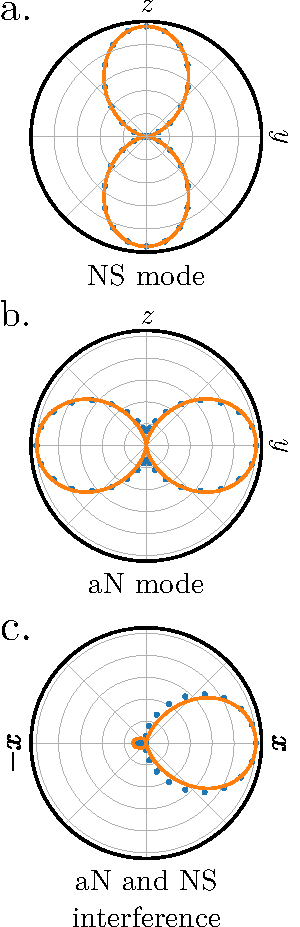
\includegraphics{fig3.pdf}
\caption{Differential radiative power profiles of the (a) NS and (b) aN magnetic plasmon resonances of the $N$-mer as well as (c) their interference as dictated by Eq. (\ref{dp_dipoles_1}). In all cases, the $N$-mer is oriented to lie in the $x-y$ plane so that the net electric dipole moment of the NS mode points along the $y$ axis and the net magnetic dipole moment of the aN mode points along the $z$ axis.}%For this geometry, the forward/backward directions refer to positive/negative $x$ direction.}
\label{scattering}
\end{centering}
\end{figure}
%%%%%%%%%%%%%%%%%%%%%%%%%%%%%%%%%%%%%%%%%%%%%%%%%%%%%%%%%%%%%%%%%%
Fig. \ref{scattering} displays the differential scattering power profiles associated with the aN (a) and NS (b) magnetic plasmon resonances as well as their interference (c) for any $N$-mer with electric and magnetic dipoles oriented as described above. Since the aN mode has only a $z$-oriented magnetic dipole, its radiation pattern is orthogonal to that of the $y$-directed electric dipole of the NS mode. This means that asymmetry in the radiation pattern is due to the excitation of both modes. Thus, examination of the radiation directionality allows one to determine the net electric or magnetic dipole character. Such forward/backward scattering asymmetries have been predicted and demonstrated in metal-semiconductor core-shell nanoparticle assemblies, that similarly exploit the interference between electric and magnetic plasmons to direct light \cite{Kivshar2012}.


Recent studies have demonstrated the utility of angle-resolved CL spectroscopy to characterize plasmon resonances in noble metal nanoparticles\cite{Coenen2011,CoPol2011,Polman2014}. Using an electron microscope fitted with a parabolic mirror, emitted CL radiation can be collected across a large portion of the backward scattering hemisphere\cite{Coenen2011,CoPol2011,Polman2014}. Here we show that with the selection rules imposed by the location of the electron beam and the specific directionality of light emission, the size-dependent spectral order of the $N$-mers' magnetic plasmon modes can be observed in angle-resolved CL spectra. 


%More specifically, based upon the selection rules imposed by the electron beam and the directionality of CL radiation, it is possible to distinguish the magnetic modes and their spectral ordering as a function of size.



%%%%%%%%%%%%%%%%%%%%%%%%%%%%%%%%%%%%%%%%%%%%%%%%%%%%%%%%%%%%%%%%%%%%%
\begin{figure}
\begin{centering}
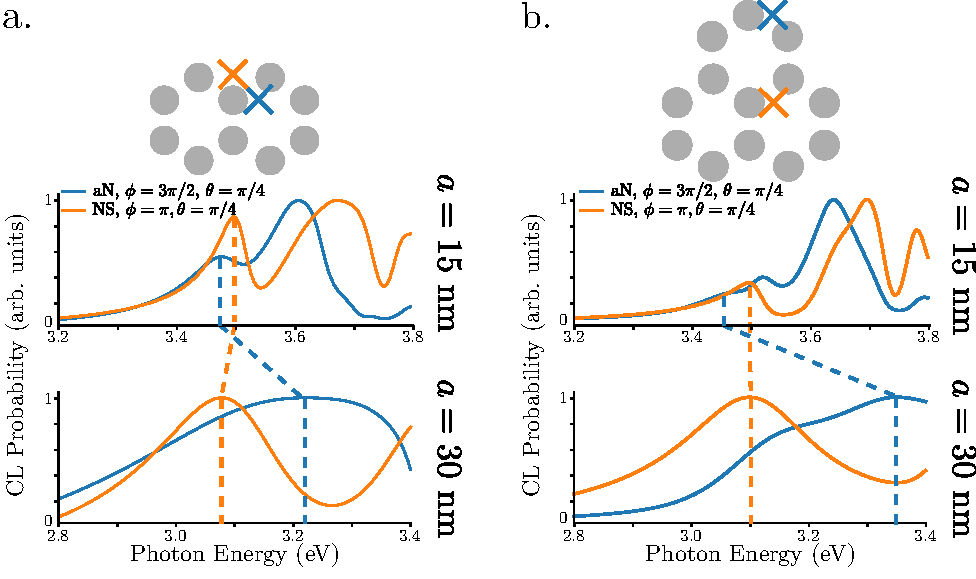
\includegraphics{fig4.pdf}
\caption{Angle-resolved cathodoluminescence spectra of the 2-mer (a) and 3-mer (b). Choosing the electron beam positions ($\times$) together with the light collection angles indicated allows the individual magnetic plasmon resonances and their size-dependent spectral switching to be observed. Simulated CL spectra with $a=15$ nm show the aN modes lower in energy than the NS modes, as predicted. With $a= 30$ nm, the modes switch in accordance with the presented coupled-dipole model. Spectral peaks located at higher energies correspond to higher-order non-magnetic plasmon modes that are not explicitly studied here.}
\label{CL_2mer_3mer}
\end{centering}
\end{figure}
%%%%%%%%%%%%%%%%%%%%%%%%%%%%%%%%%%%%%%%%%%%%%%%%%%%%%%%%%%%%%%%%%%%%%
The previous section built up intuition on the directionality of light scattered by the magnetic modes of the 2-mer and 3-mer. This intuition informs the particular angles at which to collect CL spectra. Fig. \ref{CL_2mer_3mer} shows simulated point angle-resolved CL spectra of the 2-mer and 3-mer, with the electron beam position chosen so as to excite the aN (blue) and NS (orange) modes. Note however, due to the symmetry of the oligomers, the blue electron beam position excites not only the aN mode, but also weakly the NS mode. Since the radiation profile of the aN mode is orthogonal to that of the NS mode, it is possible to distinguish them by analyzing the angular distribution of emitted CL radiation, even though their splitting is $<0.05$ eV. The angle-resolved CL spectra at two such angles are reported in Fig. \ref{CL_2mer_3mer}. These simulated spectra confirm the predictions of the model displayed in Fig. \ref{scaling}; specifically, between $a = 15 - 30$ nm, the aN and NS modes switch spectral order. The simulation also shows mode switching at $a\approx7$ nm, however, the splitting energies are too small to be experimentally detectable with conventional CL. Nevertheless, experimental confirmation of the secondary mode splitting is possible, and would verify both our analytical and numerical predictions.










\section{Magnetic Plasmon Resonances in Hexagonally-Packed Nanoclusters}
Ref. \cite{Engheta2017} synthesizes, fabricates, and optically characterizes hexagonally-packed nanoclusters composed of gold nanoparticles in the intermediate size regime, between few particle nanoclusters and infinite arrays. Here, we apply our analytical modeling and numerical simulation to investigate the behavior of magnetic plasmon resonances in silver nanoclusters of the same geometry as a function of size, with an eye toward engineering magnetic resonances at particular resonance energies. Such tunability may be important in the design of future negative index materials with spectral tunability. Specifically, we consider hexagonally packed clusters composed of 13, 19, and 31 MNPs displayed in Fig. \ref{kagan_fields} as well as the insets of Fig. \ref{kagan_eigen}.




%%%%%%%%%%%%%%%%%%%%%%%%%%%%%%%%%%%%%%%%%%%%%%%%%%%%%%%%%%%%%%%%%
\begin{figure}
\begin{centering}
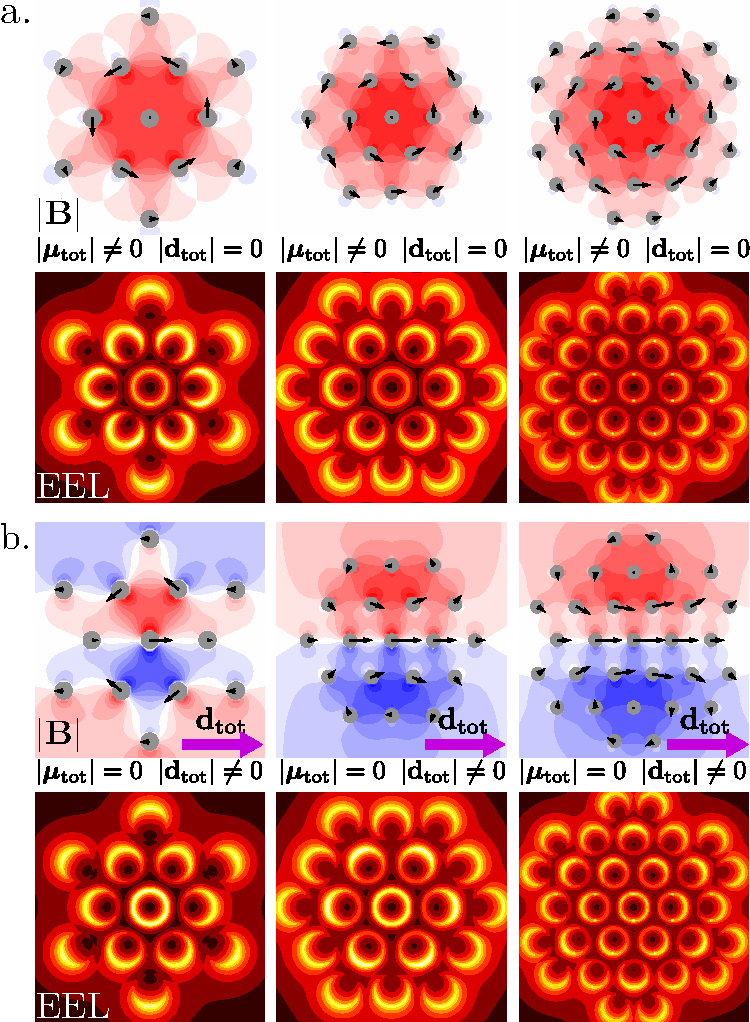
\includegraphics{fig5.pdf}
\caption{Signed magnetic field magnitudes and EEL mode maps of the aN (a) and NS (b) magnetic plasmon modes of 13-, 19-, and 31-particle nanoclusters. The clusters are based on those characterized in Ref. \cite{Engheta2017}, but are composed of silver. The magnetic fields are computed from the coupled-dipole model, while EEL mode maps result from simulation. As with the $N$-mers, only the NS modes have a net electric dipole moment indicated by the magenta arrow. The EEL mode maps indicate those regions in space where it is most probable to excite each magnetic plasmon.}
\label{kagan_fields}
\end{centering}
\end{figure}
%%%%%%%%%%%%%%%%%%%%%%%%%%%%%%%%%%%%%%%%%%%%%%%%%%%%%%%%%%%%%%%%%
Fig. \ref{kagan_fields} displays the signed magnetic field magnitude of the aN (panel a) and NS (panel b) magnetic plasmon resonances of the 13-, 19-, and 31-particle nanoclusters. The black arrows denote the electric dipole moments of the individual MNPs within each magnetic plasmon mode, the magenta arrows denote the net electric dipole moment of the nanocluster, and the background color denotes the strength of the associated magnetic field. The net electric or magnetic dipole magnitude is denoted below each panel. The lower rows of panels a and b display the energy-filtered electron energy-loss (EEL) profiles of these modes. It is important to note that each aN mode is weakly excitable from the middle MNP (as indicated by the low EEL probability surrounding it), while the NS mode is strongly excitable from the same location (as indicated by the high EEL probability surrounding it). In all cases, the NS mode is doubly degenerate as would be true of any structure with sixfold symmetry. In analogy to the oligomers, these magnetic modes are chosen because they are the simplest (i.e., lowest order) and their radiation patterns are spatially orthogonal. 



%%%%%%%%%%%%%%%%%%%%%%%%%%%%%%%%%%%%%%%%%%%%%%%%%%%%%%%%%%%%%%%%%%%%%%
\begin{figure}
\begin{centering}
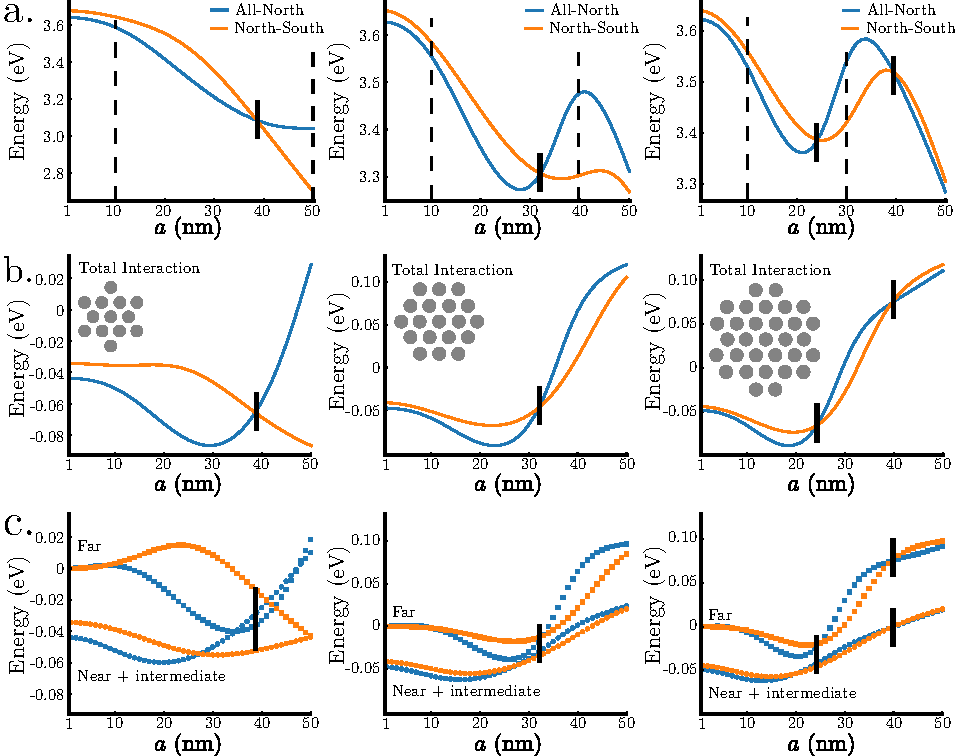
\includegraphics{fig6.pdf}
\caption{Magnetic plasmon resonance energies (a) and electric-dipole interaction energies (b,c) of 13-, 19-, and 31-particle nanoclusters similar to those characterized in Ref. \cite{Engheta2017}, but composed of silver. Due to the geometrical differences between these nanoclusters and the $N$-mers, the aN modes remain lowest in energy at small MNP radii $a$. However, as $a$ increases, one or even multiple magnetic plasmon resonance crossings become possible for the same reasons described earlier for the $N$-mers.}
\label{kagan_eigen}
\end{centering}
\end{figure}
%%%%%%%%%%%%%%%%%%%%%%%%%%%%%%%%%%%%%%%%%%%%%%%%%%%%%%%%%%%%%%%%%%%%%%
Fig. \ref{kagan_eigen} displays the evolution of the aN and NS magnetic resonances with size $a$ as dictated by the coupled-dipole model. Here the size-dependent behavior of the nanocluster resonances is different due to the hexagonal packing as opposed to the open-ring structure of the $N$-mer. Nevertheless, the model is capable of predicting the magnetic spectrum. Most surprising is the oscillatory behavior of the nanoclusters' magnetic resonances with size as opposed to the expected monotonic red-shifting of those of the $N$-mer (see Fig. \ref{scaling}). Panels b and c display the total interaction energy $U$, and its near-, intermediate-, and far-field contributions, showing that this oscillatory behavior is due to retardation effects through the $e^{ikr_{ij}}$ factor in the electric field of each electric dipole.



%This is contrary to intuition where increasing size causes monotonic redshifting. However this oscillatory behavior is not so unexpected; separating a MNP dimer causes its hybridized electric plasmon resonance frequencies to oscillate from bonding to anti-bonding and back\cite{vonPlessen2007}. In these nanoclusters, ARCL and patterns spectra provide a means to demonstrate this oscillation.






%%%%%%%%%%%%%%%%%%%%%%%%%%%%%%%%%%%%%%%%%%%%%%%%%%%%%%%%%%%%%%%%%%%%%%
\begin{figure}
\begin{centering}
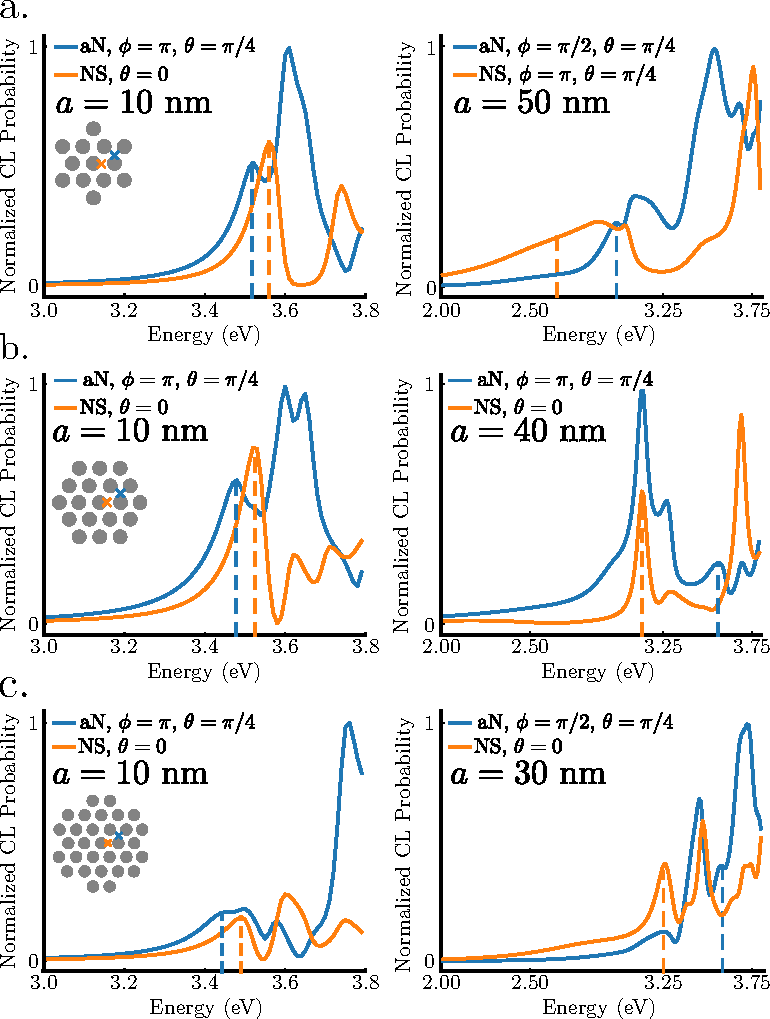
\includegraphics{fig7.pdf}
\caption{Simulated angle-resolved cathodoluminescence spectra of the (a) 13-, (b) 19-, and (c) 31-particle nanoclusters from Ref. \cite{Engheta2017}, but composed of silver. Blue (orange) spectra are acquired at the beam positions marked with a blue (orange) $\times$ to preferentially excite the aN ($x$-polarized NS) mode. The dashed lines in each spectrum indicate the resonance locations of the aN (blue) and NS (orange) modes. Each panel also displays the light collection angles associated with each spectrum. Again, all unlabeled resonance peaks correspond to higher-order plasmon modes of either electric or magnetic character, which are not studied herein.}
\label{kagan_CL}
\end{centering}
\end{figure}
%%%%%%%%%%%%%%%%%%%%%%%%%%%%%%%%%%%%%%%%%%%%%%%%%%%%%%%%%%%%%%%%%%%%%%
Fig. \ref{kagan_CL} shows simulated angle-resolved CL spectra for the 13-, 19-, and 31-particle nanoclusters acquired at the two indicated beam positions and collection angles. Inspection of the EEL maps of the NS and aN magnetic resonances in Fig. \ref{kagan_fields} indicates the optimal electron beam positions to excite each magnetic plasmon mode, i.e., those positions with highest EEL probability. In particular, the NS mode (Fig. \ref{kagan_fields}b) is most easily excited near the central MNP, while the aN mode (Fig. \ref{kagan_fields}a) is more easily excited from the outer MNPs surrounding the central MNP. Upon selecting the appropriate excitation location, the radiative profile of each mode further helps identify the two magnetic resonances of interest. Because the aN mode radiates strongly in the $x-y$ plane, and weakly in the $z$-direction, it is detectable at angles between $0 < \theta \leq \pi/2$ for all $\phi$. Alternatively, by alignment with the $x$-axis, the NS mode is detectable at angles between $0 \leq \theta < \pi/2$ and $0<\phi<\pi,$ and $\pi<\phi<2\pi.$ The aN beam position also weakly excites the degenerate NS modes, meaning the corresponding CL spectrum will provide a secondary signature of the spectral location of that mode. This fact is evident in multiple simulated CL spectra displayed in Figs. \ref{CL_2mer_3mer} and \ref{kagan_CL}, demonstrating again the ability of angle-resolved CL to distinguish between resonances split by $\lesssim0.05$ eV.




\section{Conclusion}
In conclusion, we have presented a coupled-dipole model of MNP oligomers and hexagonally-packed nanoclusters that includes the effects of retardation and use it to show that the spectral ordering of their magnetic plasmon resonances can be controllably tuned as a function of cluster size and morphology. Full-wave numerical simulation is used to confirm the prediction that magnetic plasmon resonances can even be made to switch energy order, offering a relatively facile way to modify the system's magnetic responses in an experiment. The presented analysis is especially important in elucidating the intermediate-size regime in between individual single-ring and extended two-dimensional nanocluster networks, where retardation effects can significantly modify the spectrum. We further study the angular-dependence of the power emitted from the nanoclusters and demonstrate that the aN and NS magnetic plasmon modes, as well as their size- and morphology-dependent spectral order, can be detected in angle-resolved CL. Taken together, our work not only clarifies the rich optical and magnetic behavior of noble metal nanoclusters in the intermediate-size regime, but also suggests a strategy to design negative-index plasmonic metamaterials with multiple tunable resonances in the visible spectrum.





\section{Methods}
\noindent{\it{Coupled-dipole model.}} Refs. \cite{Cherqui2014,ARPC} describe how to map the solutions of Maxwell's equations for electric plasmon resonances onto mechanical oscillators with effective masses. Based on this approach, the resulting Hamiltonian for a system of $n$ frictionless coupled oscillators is
\begin{equation}
H = \sum_{i}\frac{\textbf{p}_i^2}{2m_{\textrm{sp}}}+\frac{1}{2}m_{\textrm{sp}}\omega_{\textrm{sp}}^2\textbf{q}_i^2 - \frac{e}{2}\sum_{ij (i\neq j)}\textbf{q}_i\cdot\textbf{E}_j(\textbf{r}_i),
\label{hammy}
\end{equation}
where ${\bf q}_i$ and $\textbf{p}_i$ are the coordinate and momentum of the $i$th plasmon oscillator located at ${\bf r}_i$ with effective mass $m_{\textrm{sp}}$ and resonance frequency $\omega_{\textrm{sp}}$, defined previously. $\textbf{E}_j(\textbf{r}_i)$ is the full electric dipole field. The resulting equations of motion are,
\begin{equation}
\ddot{\textbf{q}}_i = -\omega_{\textrm{sp}}^2\textbf{q}_i + \frac{e}{m_{\textrm{sp}}}\sum_{j\neq i}\textbf{E}_j(\textbf{r}_i,\omega)
\label{equation_of_motion_again}
\end{equation}
which is Eq. (\ref{equation_of_motion}). Assuming sinusoidal oscillation in time and rewriting the electric field in terms of the plasmon coordinate results in the equations of motion
\begin{equation}
(\omega_{\textrm{sp}}^2-\omega^2)\textbf{q}_i -\frac{e^2}{m_\textrm{sp}}\sum_{j\neq i}\boldsymbol{\Lambda}_{ij}(\omega)\cdot\textbf{q}_j = 0.
\label{fourier_eom}
\end{equation}
It is this system of equations for the plasmon oscillator coordinates that we solve to determine the magnetic plasmon resonances. Considering $n=2$ identical, coupled, collinear oscillators as an example and projecting out the directional-dependence, Eq. (\ref{fourier_eom}) becomes
\begin{equation}
\begin{split}
(\omega_{\textrm{sp}}^2-\omega^2)q_1 -g_{12}(\omega)q_2 &= 0\\
(\omega_{\textrm{sp}}^2-\omega^2)q_2 -g_{12}(\omega)q_1 &= 0,
\label{fourier_eom_12}
\end{split}
\end{equation}
or, equivalently,
\begin{equation}
\begin{bmatrix}
\omega_{\textrm{sp}}^2-\omega^2 & -g_{12}(\omega)\\
-g_{12}(\omega) & \omega_{\textrm{sp}}^2-\omega^2
\end{bmatrix}
\begin{bmatrix}
q_1\\
q_2
\end{bmatrix}
=
\begin{bmatrix}
0\\
0
\end{bmatrix}.
\label{eom_matrix}
\end{equation}
where $g_{12}=-2e^2[r_{12}^{-3} - ikr_{12}^{-2}]e^{ikr_{12}}/\varepsilon_bm_{\textrm{sp}}.$ Note that the far-field contribution to $g_{12}$ vanishes here due to the assumed collinear arrangement of the dipoles. Solution of this system produces the hybridized plasmon resonance frequencies and modes of the dimer. Specifically, they are
\begin{equation}
\omega_{\pm} = \sqrt{\omega_{\textrm{sp}}^2 \pm g_{12}(\omega)}
\label{eigenvalues}
\end{equation}
and
\begin{equation}
q_{\pm} = \frac{1}{\sqrt{2}}\left(q_1 \pm q_2\right).
\label{eigenvectors}
\end{equation}
Note that the coupling term $g_{12}(\omega)$ is frequency dependent, meaning that the eigenvalue problem must be solved iteratively until convergence. The magnetic plasmon resonances described herein are obtained as a straightforward extension of this dimer example.




\noindent{\it{Simulation details.}} Optical and electron beam simulations were performed using the MNPBEM package \cite{Hohenester2012,Hohenester2014}. Each spherical nanoparticle was discretized into 144 surface elements, each assigned the following Drude model parameters for silver: $\varepsilon_{\infty} = 3.77$, $\hbar\gamma = 0.05$ eV, and $\hbar\omega_{p} = 9.15$ eV. The electron kinetic energy was chosen to be 200 keV and all calculations were performed in vacuum, i.e., $\varepsilon_{b}=1.$ The angle-resolved CL spectra were computed using standard functions within MNPBEM together with numerical angular integration through $\pm25^\circ$ about the angles $(\theta,\phi)$ indicated in the figures.


%\begin{acknowledgement}
%This work was supported by the U.S. Department of Energy Basic Energy Sciences under award number DE-SC0018040 (D.J.M.) and by the State of Washington through the University of Washington Clean Energy Institute and via funding from the Washington Research Foundation (N.P.M.). This work was facilitated through the use of advanced computational, storage, and networking infrastructure provided by the Hyak supercomputer system and funded by the STF at the University of Washington. N.P.M. would like to thank Dr. Niket Thakkar and Harrison Goldwyn for helpful discussions and advice.
%\end{acknowledgement}

% ========== CHapter 4

\chapter{Conclusion and Future Work}

The purpose of this thesis has been to theoretically characterize the optical properties of clusters of metal nanoparticles, beginning from the single MNP and building our way up from small, single clusters, to mixed-metal dimers, to fused rings, and finally to hexagonally packed arrays. Throughout all of this, we kept an eye towards real-world applications, including nanoscale fuel production and optically transparent coatings. Each of these studies was centered on simple models and intuition-building, and using that intuition to interpret experimental results and simulated experiments.

In Chapter 1, we learned about the history of nanotechnology and photonics and learned that at their intersection lies nanophotonics and plasmonics. We discussed how the time dynamics of a spherical metal nanoparticle with frequency-dependent dielectric properties is identical to those of a damped harmonic oscillator. Finally, we began to investigate how multiple MNPs interact with one another by consider the simplest possible example: two identical metal nanospheres. Through this exercise, we discovered that how we choose to model the interaction can have both qualitative and quantitative impacts on the results of calculations. Building this intuition set us up to understand the more complicated geometries of later chapters.

In Chapter 2, we examined mixed-metal, mixed geometry metal nanoclusters, specifically a gold nanoprism with a platinum sphere somewhere on its face. Modeling the nanoprism as a collection of spheres proved to be an intuitive and qualitatively useful device to better analyze the optical properties of the nanoprism. We discussed the distance- and orientation-dependence of the dipole-dipole coupling and showed that the extent to which the platinum sphere and the gold nanoprism hybridize depends very much upon their relative locations and orientations. Furthermore, we showed that hybridization can be enhanced by bringing the plasmon resonance energies closer together spectrally, as evidenced by computed electric field maps. These lessons point to facilitating energy transfer between metal nanoparticles via spatial and spectral co-location of plasmon resonances.

In Chapter 3, we looked at larger nanoparticle clusters, specifically those composed of cyclic structures. These rings of particles, sometimes called oligomers, have both the usual strong electric response of plasmonic particles and an anomalously large magnetic response, resulting from the circular hybridization of the individual electric plasmons. In the case of oligomers composed of multiple rings, properly describing retardation effects is very important, and modeling these oligomers with retardation effects shows that the magnetic resonances have dynamic spectral ordering with increasing size. We also examined hexagonally packed nanoclusters of recent experimental interest, and showed that their lowest-order magnetic plasmon resonances also exhibit dynamic spectral ordering. Because magnetic fields are, in fact, relativistic effects, it is impossible to accurately model magnetic oligomers without incorporating retardation effects.

The field of plasmonics has growing to do. It is time to move away from abstract problems and begin to apply what we have learned about how plasmonic systems behave and under what circumstances they exhibit new and monumental properties. For instance, the field of thermoplasmonics is an area of intense and possibly life-changing research. Additionally, the plasmoelectric effect has gone too long without a successful implementation. Furthermore, it is time to look into more advanced characterization methods, specfically, direct mapping of plasmon electric and magnetic fields through scanning probe or electron microscopies. In the future work section, we will discuss theoretical predictions of photon-assisted electron spectroscopies, which provide a method for characterizing a plasmon's electric fields.

\section{Future Work: Photon-Assisted Electron Spectroscopies}

The field of photon-assisted electron spectroscopies has had a recent spring. Examples of this kind of technique include Electron Energy-Gain Spectroscopy (EEGS)\cite{EEGS} , Photon-Induced Near-Electric Field Microscopy (PINEM)\cite{PINEM}, and Stimulated or Photon-Assisted Electron Energy-Loss Spectroscopy (SEELS/PAEELS)\cite{EEGS,vanAiken}. These processes involve the successive interaction of a plasmon with a photon and a relativistic electron. In the former case, the photon induces a plasmon or polarization state in the sample and the electron picks up energy from that excitation. In the latter case, the electron loses extra energy equal to the photon energy. PINEM is the bridge between these methods and describes both events. In the next section, we will investigate SEELS both quantum mechanically and classically, and attempt to bridge those approaches.\cite{AbajoRevMod,vanAiken,EEGS} This is still an active area of research and an active collaboration.

\subsection{First- and Second-order Fermi's Golden Rule}

Fermi's Golden Rule in first order takes the form
\begin{equation}
\Gamma_{fi} = \frac{2\pi}{\hbar^2}|\langle f |H_{\textrm{int}}| i \rangle |^2 \delta(\omega_f - \omega_i).
\label{FGR_1}
\end{equation}
Here, $\Gamma_{fi}$ is rate at which the system transitions from state $i$ to state $f$, $H_{\textrm{int}}$ is the interaction Hamiltonian, and the delta function enforces conservation of energy. In a system with only one perturbation or interaction, computation of the transition rate mediated by that perturbation is straightforward. However, we are interested in a system under the influence of multiple perturbations, specifically a MNP being probed both by light and by a passing electron. The choice of Fock states matters in that only certain transitions from initial states to final states are allowed and mediated by specific interactions, but for now we leave them unspecified. Allowing $H_{\textrm{int}} = H_1 + H_2$, Eq. \ref{FGR_1} becomes
\begin{equation}
\begin{aligned}
\Gamma_{fi} &= \frac{2\pi}{\hbar^2}|\langle f |H_1 + H_2| i \rangle |^2 \delta(\omega_f - \omega_i)\\
&= \frac{2\pi}{\hbar}\left[|\langle f |H_1| i \rangle + \langle f |H_2| i \rangle |^2\right] \delta(\omega_f - \omega_i)\\
& = \frac{2\pi}{\hbar}\left[|\langle f|H_1|i \rangle|^2 + |\langle f|H_2|i \rangle|^2 + \langle f|H_1|i \rangle \langle i|H_2|f \rangle + \langle f|H_2|i \rangle \langle i|H_1|f \rangle\right]\delta(\omega_f - \omega_i)
\label{FGR_1_expanded}
\end{aligned}
\end{equation}
Of course, $H_1$ and $H_2$ correspond to two different transitions, with different sets of raising and lower operators, to two different final Fock states. Because of this, the third and fourth terms of Eq. \ref{FGR_1_expanded} are necessarily zero. The two non-zero rates are mediated by $H_1$ and $H_2$ separately. If $H_1 = H_\textrm{el-pl}$ and $H_2 = H_{\textrm{ph-pl}}$, then the first rate is the EELS rate and the second rate is the absorption rate[cite Garcia de Abajo].

Fermi's Golden Rule for second order transitions looks similar to that for first order transitions:
\begin{equation}
\Gamma_{fi} = \frac{2\pi}{\hbar^4}\left|\sum_{m}\frac{\langle f |H_{\textrm{int}}| m \rangle \langle m |H_{\textrm{int}}| i \rangle }{\omega_f-\omega_i}\right|^2 \delta(\omega_f - \omega_i).
\label{FGR_2}
\end{equation}
Again the interaction Hamiltonian is a sum of perturbations, $H_{\textrm{int}} = H_1 + H_2$. Wrapping the prefactor, denominator, and delta function together into $A$ to focus on the matrix elements, the rate becomes
\begin{equation}
\begin{aligned}
\Gamma_{fi} &= A|\langle f |H_1 + H_2| m \rangle \langle m |H_1 + H_2| i \rangle|^2\\
&= A|(\langle f |H_1| m \rangle + \langle f |H_2| m \rangle) (\langle m |H_1| i \rangle + \langle m |H_2| i \rangle)|^2\\
&= A(|\langle f |H_1| m \rangle \langle m |H_1| i \rangle|^2 + |\langle f |H_2| m \rangle \langle m |H_2| i \rangle|^2\\
&+ |\langle f |H_1| m \rangle \langle m |H_2| i \rangle|^2 + |\langle f |H_2| m \rangle \langle m |H_1| i \rangle|)^2
\label{FGR_2_2}
\end{aligned}
\end{equation}
For the same reasons as in the discussion of the first order rates, the cross-terms not shown are equal to zero, because $H_1$ and $H_2$ correspond to different transitions with different intermediate and final states. If we now let $H_1 = H_\textrm{el-pl}$ and $H_2 = H_{\textrm{ph-pl}}$, the first term is $\Gamma_{\textrm{EELS}}^{(2)}$, the second term is $\Gamma_{\textrm{abs}}^{(2)}$, the third term is $\Gamma_{\textrm{EEGS}}$, and the final term is $\Gamma_{\textrm{CL}}$.

\section{SEELS from Fermi's Golden Rule}
SEELS, or Stimulated Electron Energy-Loss Spectroscopy, is a process by which a swift electron in an electron microscope loses energy to a sample that has been previously excited or polarized by light. In EELS without a light source, the electron interacts only with its own self-induced polarization in the sample. Incorporation of a light source allows the electron to interact with the superposition of fields in the sample, or equivalently, with the superposition of surface charge and current densities. We would like to show that this approach is consistent with Fermi's golden rule\cite{vanAiken,EEGS}.

We define the overall SEELS rate as a sum of a second order rate (photon absorption followed by electron interaction) with a first order rate (the photon-less EELS rate). This is because if the photon field (or laser intensity) is reduced to zero, the SEELS rate should reduce to the EELS rate. To evaluate the rates, we begin with an initial Fock state defined by $|k_0N_i0_l\rangle$, corresponding to an electron with wavenumber $k_0$ and frequency $\varepsilon_{k_0}$, $N$ photons of energy $\hbar\omega_i$, and zero plasmons in mode $l$ with complex frequency $\tilde{\omega}_{\textrm{pl}}=\omega_{\textrm{pl}}+\textrm{i}\gamma_{\textrm{pl}}$. We also begin at the level of the probability by multiplying the rate by $L/v$, the electron quantization length divided by the electron's velocity.
\begin{align}
\begin{split}
  P_{\textrm{SEELS}} &= \frac{2\pi L}{\hbar^4v}\left|\frac{\langle k(N-1)_i2_l|H_{\textrm{e-pl}}|k_0(N-1)_i1_l\rangle\langle k_0(N-1)_i1_l|H_{\textrm{ph-pl}}|k_0N_i0_l\rangle}{\omega_i - \tilde{\omega}_{\textrm{pl}}}\right|^2\delta(\varepsilon_k - \varepsilon_{k_0}-\omega_i)\\
  &+ \frac{2\pi L}{\hbar^2v}|\langle kN_i1_l|H_{\textrm{e-pl}}|k_0N_i0_l\rangle|^2\delta(\epsilon_k - \epsilon_{k_0} - 2\tilde{\omega}_{\textrm{pl}} + \hbar\omega_i)
  \label{overall_rate}
  \end{split}
\end{align}
Here, we have chosen the intuitive intermediate and final state for this transition. The first term is the second-order process and the second term is the first-order process which shall eventually become the EELS rate. Additionally, our interaction Hamiltonians can be defined as
\begin{equation}
\begin{aligned}
H_{\textrm{e-pl}} = -\textbf{d} \cdot \textbf{E}_{\textrm{el}}&\\
H_{\textrm{ph-pl}} = -\textbf{d} \cdot \textbf{E}_{\textrm{ph}}&
\end{aligned}
\end{equation}
with the transition dipole moment $\textbf{d} = \textbf{d}_0(b + b\dagger)$, the photon electric field with frequency $\omega_i$ and quantization volume $V$ is $\textbf{E}_{\textrm{ph}} = \sqrt{2\pi\hbar\omega_i/V}(a - a\dagger)$, and electron electric field $\langle k'|\textbf{E}_{\textrm{el}}|k\rangle = \textbf{E}_{\textrm{el}}(k',k)$. Plugging in these definitions and performing the ladder operations, the SEELS probability becomes
\begin{align}
\begin{split}
  P_{\textrm{SEELS}} &= \frac{2\pi L}{\hbar^4v}\left|\frac{\sqrt{2}\textbf{E}_{\textrm{el}}\cdot\textbf{d}_0 \sqrt{N}\textbf{d}_0\cdot\textbf{E}_{0}}{\omega_i - \tilde{\omega}_{\textrm{pl}}}\right|^2\delta(\varepsilon_k - \varepsilon_{k_0}-\omega_i)\\
  &+ \frac{2L}{\hbar v}|\textbf{E}_{\textrm{el}}\cdot\textbf{d}_0|^2
  \label{change_eels}
  \end{split}
\end{align}
Recognizing that $\delta(x_1 - x_2) = 1/\pi\textrm{Im}\{1/(x_1-x_2)\}$, $\alpha(\omega_i) = d_0^2/(\hbar(\omega_i-\omega_{\textrm{pl}}))$, and $\alpha(\epsilon_k-\epsilon_{k_0}) = d_0^2/(\hbar(\epsilon_k-\epsilon_{k_0}-\omega_{\textrm{pl}}))$, we can rewrite the SEELS probability in terms of the plasmonic nanoparticle polarizability.
\begin{align}
\begin{split}
  P_{\textrm{SEELS}} &= \frac{4\pi NL}{\hbar^2v}(\textbf{E}_{\textrm{el}}\cdot\alpha^*\cdot\textbf{E}_{\textrm{el}}^*)(\textbf{E}_0\cdot\alpha\cdot\textbf{E}_0^*)\delta(\varepsilon_k - \varepsilon_{k_0}-\omega_i)\\
  &+ \frac{2L}{\hbar v}(\textbf{E}_{\textrm{el}}\cdot\textrm{Im}\{\alpha\}\cdot\textbf{E}_{\textrm{el}}^*)
  \label{seels_with_polar}
  \end{split}
\end{align}

We will soon determine the SEELS rate via three different approaches. Before that, however, we will do some quick complex algebra that will help us determine what to do with the interaction energy terms in the SEELS rate.
\begin{equation}
\begin{aligned}
\textbf{E}\cdot\alpha\cdot\textbf{E}^* &= (\textbf{E}_r+\textrm{i}\textbf{E}_i)\cdot(X+\textrm{i}Y)\cdot(\textbf{E}_r-\textrm{i}\textbf{E}_i)\\
& = (X\textbf{E}_r - Y\textbf{E}_i + \textrm{i}X\textbf{E}_i + \textrm{i}Y\textbf{E}_r)\cdot(\textbf{E}_r-\textrm{i}\textbf{E}_i)\\
& = X(E_r^2 + E_i^2) + \textrm{i}Y(E_r^2 + E_i^2)
\label{alpha_1}
\end{aligned}
\end{equation}
and similarly 
\begin{equation}
\textbf{E}\cdot\alpha^*\cdot\textbf{E}^* = X(E_r^2 + E_i^2) -\textrm{i}Y(E_r^2 + E_i^2)
\label{alpha_2}
\end{equation}
This allows us to finally write the SEELS probability as
\begin{align}
\begin{split}
  P_{\textrm{SEELS}} &= \frac{4\pi NL}{\hbar^2v}|\alpha|^2|\textbf{E}_{\textrm{el}}|^2|\textbf{E}_{\textrm{ph}}|^2\delta(\varepsilon_k - \varepsilon_{k_0}-\omega_i)\\
  &+ \frac{2L}{\hbar v}\textrm{Im}\{\textbf{E}_{\textrm{el}}\cdot\alpha\cdot\textbf{E}_{\textrm{el}}^*\}
  \label{alpha_squared}
  \end{split}
\end{align}

The second term of Eq. \ref{alpha_squared} is the EELS probability. We now want to compute the rate from the probability. To do that, we will take the following integral and assume the no-recoil limit ($\epsilon_k - \epsilon_{k_0} = v(k-k_0) = vk'$)
\begin{equation}
\Gamma_{\textrm{SEELS}} = \frac{L}{2\pi}\int dk' P_{\textrm{SEELS}} \delta(v(k')-\omega)
\label{prob_to_rate}
\end{equation}

The delta function simply allows the replacement of all $k' = k-k_0$ with $\omega/v$. Now, writing down both $\textbf{E}_{\textrm{el}}$ and $\textbf{E}_{\textrm{ph}}$, the SEELS rate becomes
\begin{equation}
\begin{aligned}
\Gamma_{\textrm{SEELS}} &= \frac{8e^2\omega^2}{\hbar^3v^4\gamma_{L}^4}\left[\gamma_{L}^2K_1^2\left(\frac{\omega R}{v\gamma_L}\right)+K_0^2\left(\frac{\omega R}{v\gamma_L}\right)\right]\left(\frac{2\pi N\hbar\omega_i}{V}\right)|\alpha|^2\delta(\omega-\omega_i) + \Gamma_{\textrm{EELS}}\\
& = \frac{16\pi e^2\omega^2 I_0}{\hbar^3v^4\gamma_{L}^4}\left[\gamma_{L}^2K_1^2\left(\frac{\omega R}{v\gamma_L}\right)+K_0^2\left(\frac{\omega R}{v\gamma_L}\right)\right]|\alpha|^2\delta(\omega-\omega_i) + \Gamma_{\textrm{EELS}}\\
& = 2\Gamma_{\textrm{EEGS}} + \Gamma_{\textrm{EELS}}.
\label{seels_eegs}
\end{aligned}
\end{equation}
Thus, the SEELS rate is twice the EEGS rate plus the EELS rate. We have recently implemented this definition of SEELS using the MNPBEM toolbox\cite{Hohenester2012,Hohenester2014}, as shown in figure blah.

[FIGURE]

We could also try to write the SEELS rate in terms of first-order rates. To do so, we must start from the probability and split the polarizability into its real and imaginary parts. Starting from Eq. \ref{seels_prob_with_alpha} and using the identities in Eq. \ref{alpha_1} and \ref{alpha_2}, we can rewrite the SEELS probability into three terms.
\begin{equation}
\begin{split}
  P_{\textrm{SEELS}} &= \frac{4\pi NL}{\hbar^2v}(\textbf{E}_{\textrm{el}}\cdot\textrm{Im}\{\alpha\}\cdot\textbf{E}_{\textrm{el}}^*)(\textbf{E}_0\cdot\textrm{Im}\{\alpha\}\cdot\textbf{E}_0^*)\delta(\varepsilon_k - \varepsilon_{k_0}-\omega_i)\\
  &+ \frac{2L}{\hbar v}(\textbf{E}_{\textrm{el}}\cdot\textrm{Im}\{\alpha\}\cdot\textbf{E}_{\textrm{el}}^*)\\
  &+ \frac{4\pi NL}{\hbar^2v}(\textbf{E}_{\textrm{el}}\cdot\textrm{Re}\{\alpha\}\cdot\textbf{E}_{\textrm{el}}^*)(\textbf{E}_0\cdot\textrm{Re}\{\alpha\}\cdot\textbf{E}_0^*)\delta(\varepsilon_k - \varepsilon_{k_0}-\omega_i)
  \label{seels_prob_with_alpha}
  \end{split}
\end{equation}
From here, we again convert $P_{\textrm{SEELS}}$ to $\Gamma_{\textrm{SEELS}}$ using Eq. \ref{prob_to_rate}.
\begin{equation}
\begin{split}
  \Gamma_{\textrm{SEELS}} &= \frac{8 e^2 \omega^2}{\hbar^3v^4\gamma_L^4}\left[\gamma_{L}^2K_1^2\left(\frac{\omega R}{v\gamma_L}\right)+K_0^2\left(\frac{\omega R}{v\gamma_L}\right)\right]\textrm{Im}\{\alpha\}\left(\frac{2\pi N\hbar\omega_i}{V}\right)\textrm{Im}\{\alpha\}\delta(\omega-\omega_i)\\
  &+ \frac{8 e^2 \omega^2}{\hbar^3v^4\gamma_L^4}\left[\gamma_{L}^2K_1^2\left(\frac{\omega R}{v\gamma_L}\right)+K_0^2\left(\frac{\omega R}{v\gamma_L}\right)\right]\textrm{Re}\{\alpha\}\left(\frac{2\pi N\hbar\omega_i}{V}\right)\textrm{Re}\{\alpha\}\delta(\omega-\omega_i)\\
  &+ \Gamma_{\textrm{EELS}}
  \label{seels_rate_split}
  \end{split}
\end{equation}
Again, using the definitions given by Garcia de Abajo[cite Garcia de Abajo], we can rewrite the SEELS rate in terms of first order probabilites.
\begin{equation}
\begin{split}
  \Gamma_{\textrm{SEELS}} &= \frac{\sigma_{\textrm{ext}}I_0}{\hbar\omega_i}\Gamma_{\textrm{EELS}}\delta(\omega-\omega_i)\\
  &+ \frac{8 e^2 \omega^2}{\hbar^3v^4\gamma_L^4}\left[\gamma_{L}^2K_1^2\left(\frac{\omega R}{v\gamma_L}\right)+K_0^2\left(\frac{\omega R}{v\gamma_L}\right)\right]\textrm{Re}\{\alpha\}\left(\frac{2\pi N\hbar\omega_i}{V}\right)\textrm{Re}\{\alpha\}\delta(\omega-\omega_i)\\
  &+ \Gamma_{\textrm{EELS}}
  \label{seels_rate_first}
  \end{split}
\end{equation}
Of course, the real parts come along for the ride, since they are unrelated to any particular first-order rate. We could recombine the real parts and the imaginary parts to recover Eq. \ref{seels_eegs}. 

At the level of Eq. \ref{seels_prob_with_alpha}, we could also rewrite each term such that it contains a complex-valued dipole moment, either $\textbf{d}_{\textrm{el}}$ or $\textbf{d}_{\textrm{ph}}$. To do this we again need to do some complex algebra.
\begin{equation}
\begin{aligned}
P_{\textrm{SEELS}} &= \frac{4\pi NL}{\hbar^2v}(\textbf{E}_{\textrm{el}}\cdot\alpha^*\cdot\textbf{E}_{\textrm{el}}^*)(\textbf{E}_0\cdot\alpha\cdot\textbf{E}_0^*)\delta(\varepsilon_k - \varepsilon_{k_0}-\omega_i)\\
  &+ (-\textrm{i})\frac{2L}{\hbar v}(\textbf{E}_{\textrm{el}}\cdot\alpha\cdot\textbf{E}_{\textrm{el}}^*-\textbf{E}_{\textrm{el}}\cdot\textrm{Re}\{\alpha\}\cdot\textbf{E}_{\textrm{el}}^*)
  \label{real_alphas}
\end{aligned}
\end{equation}
Here, we have multiple terms which contain a complex-valued polariability. Recalling that $\textbf{d}_{\textrm{el,ph}} = \alpha\textbf{E}_{\textrm{el,ph}}$, we can write the SEELS probability as a sum of induced dipole moments
\begin{equation}
\begin{aligned}
P_{\textrm{SEELS}} &= \textbf{E}_{\textrm{el}}^*\cdot\left\{\frac{4\pi NL}{\hbar^2v}\textbf{d}_{\textrm{ph}}(\textbf{E}_{\textrm{el}}\cdot\textbf{d}_{\textrm{ph}}^*)\delta(\varepsilon_k - \varepsilon_{k_0}-\omega_i) - \frac{2L\textrm{i}}{\hbar v}\textbf{d}_{\textrm{el}}\right\}\\
  &+ \frac{2L\textrm{i}}{\hbar v}\textrm{Re}\{\textbf{E}_{\textrm{el}}^*\cdot\textbf{d}_{\textrm{el}}\}.
  \label{seels_dipoles}
\end{aligned}
\end{equation}
Again, the extra real part comes along for the ride.

\subsection{A Classical Description of EELS (and SEELS)}

A common way to compute the EELS rate is by calculating the induced field of the plasmon and having it act on the passing electron via\cite{AbajoRevMod,Hohenester2014,Quillin} [cite Garcia de Abajo ]
\begin{equation}
\Gamma_{\textrm{EELS}}(\textbf{r},\omega) = \frac{e}{\pi\hbar\omega}\int dt \textrm{Re}\left\{ e^{-\textrm{i}\omega t} \textbf{v} \cdot \textbf{E}_{\textrm{ind}}(\textbf{r},\omega)\right\}.
\label{eels_rate_bem_1}
\end{equation}
Here, $\textbf{v}$ is the velocity of the electron. It will, however, be more convenient to write the EELS rate in terms of the electron electric field and the induced dipole moment of the plasmon. First, the induced field is written in terms of induced potentials
\begin{equation}
\begin{aligned}
\textbf{E}_{\textrm{ind}} &= -\nabla\phi_{\textbf{ind}} - \frac{\dot{\textbf{A}}_{\textrm{ind}}}{c}\\
&= -\nabla\phi_{\textrm{ind}} + \textrm{i}k\textbf{A}_{\textrm{ind}}.
\label{field_induced}
\end{aligned}
\end{equation}
The induced scalar potential $\phi_{\textrm{ind}}$ and vector potential $\textbf{A}_{\textrm{ind}}$ are related to the induced charge and current densities, respectively
\begin{equation}
\begin{aligned}
&\phi(\textbf{x},\omega) = \int d^3x' \frac{e^{\textrm{i}k|\textbf{x}-\textbf{x}'|}}{|\textbf{x}-\textbf{x}'|}\rho(\textbf{x}',\omega)\\
&\textbf{A}(\textbf{x},\omega) = \int d^3x' \frac{e^{\textrm{i}k|\textbf{x}-\textbf{x}'|}}{|\textbf{x}-\textbf{x}'|}\frac{\textbf{J}(\textbf{x}',\omega)}{c}.
\label{potentials}
\end{aligned}
\end{equation}
Defining $t = z/v$, $dt = dz/v$, and $q = \omega/v$, and plugging Eq. \ref{potentials} and \ref{field_induced} into Eq. \ref{eels_rate_bem_1}, the EELS rate becomes
\begin{equation}
\Gamma_{\textrm{EELS}} = \frac{e}{v\pi\hbar\omega}\int dz \textrm{Re}\left\{ e^{-\textrm{i}qz} \textbf{v} \cdot \left[\int d^3x' \left(-\nabla\frac{e^{\textrm{i}k|\textbf{x}-\textbf{x}'|}}{|\textbf{x}-\textbf{x}'|}\rho(\textbf{x}',\omega)\right) + \textrm{i}k\left(\frac{e^{\textrm{i}k|\textbf{x}-\textbf{x}'|}}{|\textbf{x}-\textbf{x}'|}\frac{\textbf{J}(\textbf{x}',\omega)}{c}\right)\right]\right\}.
\label{eels_with_potentials}
\end{equation}
Defining the Green's function $e^{\textrm{i}k|\textbf{x}-\textbf{x}'}/|\textbf{x}-\textbf{x}'| = 4\pi G(\textbf{x},\textbf{x}')$ allows us to write down a pseudo-potential $\psi = \int dz e^{-\textrm{i}qz} G(\textbf{x},\textbf{x}')$. Integrating by parts deals with the gradient in Eq. \ref{eels_with_potentials} by moving it to $\psi$ as follows: 
\begin{equation}
\int dz e^{-\textrm{i}qz} \nabla G(\textbf{x},\textbf{x}') = e^{-\textrm{i}qz} G(\textbf{x},\textbf{x}') \hat{\textbf{z}} \Big|_{-\infty}^{\infty} + \textrm{i}q \psi \hat{\textbf{z}}.
\label{psi_integral}
\end{equation}
The first term on the right hand side, the surface term, is zero, so the integral of the gradient of the Green's function is simply $\textrm{i}q\psi$.

Rewriting $G$ in terms of its Fourier transform reveals a route to computing the integral in $z$. Doing so results in a new form for the pseudo-potential
\begin{equation}
\begin{aligned}
\psi &= \int dz e^{-\textrm{i}qz} G(\textbf{x},\textbf{x}')\\ 
&= \int dz e^{-\textrm{i}qz} \int \frac{d^3k'}{(2\pi)^3} \frac{4\pi}{k'^2 - k^2} e^{\textrm{i}\textbf{k}'\cdot(\textbf{x}-\textbf{x}')}\\
&= \int \frac{d^3k'}{(2\pi)^3} \frac{4\pi}{k'^2 - k^2} e^{\textrm{i}[k'_x(x-x')+k'_y(y-y')-k'_zz']} \int dz e^{-\textrm{i}(q-k'_z)z}\\
&= \int \frac{d^3k'}{(2\pi)^3} \frac{4\pi}{k'^2 - k^2} e^{\textrm{i}[k'_x(x-x')+k'_y(y-y')-k'_zz']} 2\pi\delta(q-k'_z)\\
&= \int \frac{d^3k'}{(2\pi)^3} \frac{4\pi}{k'^2 - k^2} e^{\textrm{i}\textbf{k}'\cdot(\textbf{x}_{\perp}-\textbf{x}')} 2\pi v \delta(\omega-\textbf{v}\cdot\textbf{k}').
\label{psi_k_space}
\end{aligned}
\end{equation}
We will see that through this definition of $\psi$ we can construct the electron's electric field. For now, we rewrite Eq. \ref{eels_with_potentials} in terms of $\psi$
\begin{equation}
\Gamma_{\textrm{EELS}} = \frac{4e}{v\hbar\omega}\textbf{v}\cdot\textrm{Re}\int d^3x' \psi(\textbf{x}_{\perp},\textbf{x}',\omega) \left[-\textrm{i}q\rho(\textbf{x}',\omega)\hat{\textbf{z}} + \textrm{i}k\frac{\textbf{J}(\textbf{x}',\omega)}{c}\right],
\label{eels_with_psi}
\end{equation}
and turn our attention to the induced charge and current densities. The densities are defined by an induced dipole moment, $\textbf{d}_{\textrm{ind}}$ as follows:
\begin{equation}
\begin{aligned}
\rho(\textbf{x}',\omega) = \textbf{d}\cdot\nabla_{r}\delta(\textbf{x}'-\textbf{r})&\\
\textbf{J} = \textrm{i}\omega\textbf{d}\delta(\textbf{x}'-\textbf{r})&.
\label{densities}
\end{aligned}
\end{equation} 
Plugging Eq. \ref{densities} into Eq. \ref{eels_with_psi} gives the EELS rate
\begin{equation}
\Gamma_{\textrm{EELS}} = \frac{4e}{v\hbar\omega}\textbf{v}\cdot\textrm{Re}\int d^3x' \psi(\textbf{x}_{\perp},\textbf{x}',\omega) \left[-\textrm{i}q \textbf{d}\cdot\nabla_{r}\delta(\textbf{x}'-\textbf{r})\hat{\textbf{z}} + \textrm{i}k\frac{\textrm{i}\omega\textbf{d}\delta(\textbf{x}'-\textbf{r})}{c}\right]
\label{eels_with_densities}
\end{equation}

A useful mathematical identity allows $\psi\textbf{d}\cdot\nabla_r\delta(\textbf{x}'-\textbf{r}) = \textbf{d}\cdot(\nabla_r\psi)\delta(\textbf{x}'-\textbf{r})$, and the integral over both delta functions makes the replacement $\textbf{x}' \rightarrow \textbf{r}$. In addition, taking the gradient of $\psi$ results in $\nabla_r\psi(\textbf{x}_{\perp},\textbf{r},\omega) = -\textrm{i}\textbf{k}'\psi(\textbf{x}_{\perp},\textbf{r},\omega)$. The EELS rate becomes
\begin{equation}
\Gamma_{\textrm{EELS}} = \frac{4e}{v\hbar\omega}\textbf{v}\cdot \textrm{Re}\psi(\textbf{x}_{\perp},\textbf{r},\omega) \left[(\textrm{i}q)(\textrm{i}\textbf{k}') \cdot \textbf{d}\hat{\textbf{z}} - (\textrm{i}k)(\textrm{i}k')\textbf{d}\right]
\end{equation}
The electron has momentum only in the z-direction, so $q\hat{\textbf{z}} = \textbf{q}$. Using this definition and writing out $\psi$ in full results in the following form for the EELS rate.
\begin{equation}
\begin{aligned}
\Gamma_{\textrm{EELS}} &= \frac{4e}{v\hbar\omega}\textbf{v}\cdot \textrm{Re}\int \frac{d^3k'}{(2\pi)^3} \frac{4\pi}{k'^2 - k^2} e^{\textrm{i}\textbf{k}'\cdot(\textbf{x}_{\perp}-\textbf{r})} 2\pi v \delta(\omega-\textbf{v}\cdot\textbf{k}') \left[(\textrm{i}\textbf{q})(\textrm{i}\textbf{k}') \cdot \textbf{d} - (\textrm{i}k)(\textrm{i}k)\textbf{d}\right]\\
&= \frac{4\textrm{i}e}{\pi\hbar} \textrm{Im}\int d^3q \frac{\textbf{q} - k\textbf{v}/c}{q^2 - k^2} \cdot \textbf{d} \delta(\omega - \textbf{v} \cdot \textbf{q})\\
&= \frac{4}{\hbar}\textrm{Im}\left\{ \textbf{E}_{\textrm{el}} \cdot \textbf{d}_{\textrm{ind}}\right\}.
\end{aligned}
\end{equation}
Here, since $k'$ is an integration variable, it has been rewritten as $q$ and the definition of the electron's electric field from Ref. \cite{AbajoRevMod} has been used to replace $\psi$. So, the common implementation of the EELS rate using the induced electric fields and electron velocity is entirely consistent with the method of using the induced dipole moment and electron electric field.

The MNPBEM software package computes EELS and other observables using induced surface charge and current densities\cite{Hohenester2012,Hohenester2014}. These quantities are ostensibly related to the induced dipole moments. We have implemented a method for computing SEELS that involves adding photon-induced surface charges and currents to electron-induced surface charges and currents, and using that superposition to compute the EELS rate\cite{vanAiken}. In terms of induced dipole moments, this takes the form
\begin{equation}
\Gamma_{\textrm{SEELS}} = \frac{4}{\hbar}\textrm{Im}\left\{ \textbf{E}_{\textrm{el}} \cdot (\textbf{d}_{\textrm{el}}+\textbf{d}_{\textrm{ph}})\right\}
\label{eels_dipoles}
\end{equation}
It is unclear at this point in time how Eq. \ref{seels_dipoles} relates to the Fermi's golden rule approaches from a previous section.

\subsection{SEELS from the Perspective of the Force on the Plasmon}

Ref. \cite{Quillin} computes the EELS rate through the power absorbed by the plasmon from the passing electron, using the electron's electric field to quantify the force on the plasmon. Interestingly, in the event that the plasmon is forced by both light and an electron beam simultaneously, the EELS rate becomes a more complicated loss rate. According to the definition in Ref. \cite{Quillin}
\begin{equation}
\Gamma_{\textrm{loss}}(\textbf{R},\omega) = \frac{|\textbf{F}(\textbf{R},\omega)|^2}{e^2\hbar\omega}\textrm{Im}\{\alpha_{\textrm{sp}}(\omega)\}.
\label{gamma_loss}
\end{equation}
Here, $\Gamma_{\textrm{loss}}(\textbf{R},\omega)$ is the rate of any possible energy-loss event and $\textbf{F}(\textbf{R},\omega)$ is the force on the plasmon. Assuming our plasmon oscillator is simply a dipole $\textbf{d}=e\textbf{q}$, the force on the dipole becomes $\textbf{F}(\textbf{R},\omega) = e\textbf{E}_{\textbf{tot}}(\textbf{R},\omega)$, the electron charge times the total of the electric fields acting on the plasmon. Those electric fields, in the frequency domain, are
\begin{equation}
\begin{aligned}
\textbf{E}_{\textrm{tot}}(\textbf{R},\omega) &= \textbf{E}_{\textrm{ph}}(\textbf{R},\omega) + \textbf{E}_{\textrm{el}}(\textbf{R},\omega)\\
& = 2\pi A\delta(\omega-\omega_0)\hat{\boldsymbol{\epsilon}} + \frac{2e\omega}{v^2\gamma_L^2}\left[ \textrm{i}K_0\big( \frac{\omega R}{v\gamma_L} \big)\hat{\textbf{z}} -  \gamma_L K_1\big( \frac{\omega R}{v\gamma_L} \big)\hat{\textbf{R}}\right]e^{\textrm{i}\omega z/v}.
\label{fields_sum}
\end{aligned}
\end{equation}
The photon field with polarization direction $\hat{\boldsymbol{\epsilon}}$ is scaled by the intensity of the laser, here called $A$, and in the case where the incoming light is actually a packet of frequencies around $\omega_0$ the delta function becomes a lorentzian or gaussian distribution whose width is related to the bandwidth of the optical pump. The electron electric field has been previously defined. Plugging this field into Eq. \ref{gamma_loss}, the loss rate becomes
\begin{equation}
\begin{aligned}
\Gamma_{\textrm{loss}} &= \frac{\textrm{Im}\{\alpha(\omega)\}}{\hbar\pi}\Big\{4\pi^2A^2\delta(\omega-\omega_0)\\
&+ \frac{4e^2\omega^2}{v^4\gamma_L^4}\left[K_0^2\left(\frac{\omega R}{v\gamma_L}\right) + \gamma_L^2 K_1^2\left(\frac{\omega R}{v\gamma_L}\right)\right]\\
&+ 2\pi A\delta(\omega-\omega_0)\hat{\boldsymbol{\epsilon}}\cdot\left[ \textrm{i}K_0\left( \frac{\omega R}{v\gamma_L} \right)\hat{\textbf{z}} - \gamma_L K_1\left( \frac{\omega R}{v\gamma_L} \right)\hat{\textbf{R}}\right]e^{\textrm{i}\omega z/v}\\
&+ 2\pi A\delta(\omega-\omega_0)\hat{\boldsymbol{\epsilon}}\cdot\left[ -\textrm{i}K_0\left( \frac{\omega R}{v\gamma_L} \right)\hat{\textbf{z}} - \gamma_L K_1\left( \frac{\omega R}{v\gamma_L} \right)\hat{\textbf{R}}\right]e^{-\textrm{i}\omega z/v} \Big\}.
\label{loss_rate_fields}
\end{aligned}
\end{equation}
This equation is very similar to the loss probability presented in Ref. \cite{vanAiken}. We are interested in modeling particular experimental situations, specifically experiments in which the photon and electron interact with the MNP at the same time and the light is polarized such that $\hat{\boldsymbol{\epsilon}}_0 \cdot \hat{\textbf{z}} = 0$. This reduces Eq. \ref{loss_rate_fields} to
\begin{equation}
\begin{aligned}
\Gamma_{\textrm{loss}} &= \frac{\textrm{Im}\{\alpha(\omega)\}}{\hbar\pi}\Big\{4\pi^2A^2\delta(\omega-\omega_0)\\
&+ \frac{4e^2\omega^2}{v^4\gamma_L^4}\left[K_0^2\left(\frac{\omega R}{v\gamma_L}\right) + \gamma_L^2 K_1^2\left(\frac{\omega R}{v\gamma_L}\right)\right]\\
&+ 2\textrm{Re}\left\{2\pi A\delta(\omega-\omega_0)\hat{\boldsymbol{\epsilon}}\cdot\left[ -\gamma_L K_1\left( \frac{\omega R}{v\gamma_L} \right)\hat{\textbf{R}}\right]e^{\textrm{i}\omega z/v}\right\}\Big\}
\label{loss_fields_realpart}
\end{aligned}
\end{equation}




% ==========   Appendices
%
\appendix
\raggedbottom\sloppy
 
% ========== Appendix A
\chapter{Supporting Information: Imaging Energy Transfer in Pt-Decorated Au Nanoprisms via Electron Energy-Loss Spectroscopy}

\section{General Materials and Methods}

General materials and methods. Hexadecyltrimethylammonium bromide (CTAB, 99\%), chloroplatinic acid (H2PtCl6, 8 wt. \% in H2O) hydrogen tetrachloroaurate trihydrate (HAuCl4•3H2O, 99.999\%), L-ascorbic acid (99\%), sodium borohydride (NaBH4, 99.99\%), sodium hydroxide (99.99\%), sodium iodide (NaI, 99.999\%), and trisodium citrate (99\%) were obtained from Sigma Aldrich and used as received. 11-amino-1-undecanethiol hydrochloride (AUT, 99.2\%) was purchased from Dojindo (Rockville, MD) and used as received. NANOpure™ water Thermo Scientific, > 18.2 MΩ•cm) was used for all washing, synthesis, and purification protocols as well as in the preparation of all solutions. All stock solutions were aqueous and prepared fresh before each reaction, unless otherwise noted. All glassware was washed with aqua regia (3:1 ratio of concentrated HCl and HNO3 by volume) and rinsed thoroughly with water.

\section{Au Nanoprism Synthesis}

Au nanoprisms were synthesized according to previous protocols. (1, 2) Two hours after Au nanoparticle seeds were added to the nanoprism growth solution, the reaction mixture was heated in a H2O bath to 37 °C for 1 minute to dissolve any CTAB that may have recrystallized during the growth period (this crystallized CTAB can interfere with nanoprism purification by centrifugation). To separate the nanoprisms from pseudospherical nanoparticle reaction byproducts, 90 mL of the reaction mixture was divided into 15 mL conical tubes and
centrifuged at 820 rcf for 15 minutes (Eppendorf centrifuge 5804 with swing bucket rotor A-4-44). The supernatant and pellet were both extracted and the nanoprism thin film was resuspended in 1.0 mL of H2O by vortexing for 5 seconds. To remove additional CTAB and excess reagents, this mixture was transferred to 1.5 mL centrifuge tubes, and the prisms were then centrifuged using a Spectrum minicentrifuge (SC1006-R) for approximately 5 minutes. After centrifugation, the supernatant was removed and the prisms were resuspended in 1.0 mL of H2O and subsequently combined in a 15 mL conical tube. The concentration of the purified nanoprisms in the nanoprism stock solution was then adjusted to an optical density (O.D.) of 1.0 a.u. at the maximum absorption wavelength (λmax, approximately 1300 nm) by ultraviolet-visible-near infrared (UV-vis-NIR) spectroscopy.

\section{Pt-decorated Au Nanoprism Synthesis}

To 1.0 mL of purified Au nanoprisms (absorbance at λmax = 1.0 a.u.) was added 8.0 μL of 1 mM AUT. The mixture was
vortexed, and the nanoprisms were allowed to rest for 24 hours to allow for thiol conjugation to the nanoparticle surface. After this period, 20 μL of 20 mM ascorbic acid was added, and the nanoparticle solution was vortexed briefly. Next, 20 μL of 2 mM H2PtCl6 was added, the solution was briefly vortexed, and the nanoprisms were allowed to rest for an additional 24 hours to ensure complete reduction of H2PtCl6. 

\section{UV-vis-NIR Spectroscopy}

Nanoprism solutions were analyzed by UV-vis-NIR spectroscopy using a Cary 5000 spectrophotometer (Agilent, Inc.). Baselines were collected using H2O as reference solutions.

\section{Transmission Electron Microscopy (TEM)}

Nanoparticle products were purified by centrifugation using a Spectrum mini-centrifuge (SC1006-R). After removal of the supernatant, the pellet was resuspended in 1.0 mL of H2O and the process was repeated. After subsequent removal of the supernatant, nanoprism products were resuspended in 30 μL of H2O by vortexing and sonicating for approximately 10 seconds. For general TEM imaging, a 5 μL aliquot of each concentrated nanoprism sample was dropcast onto a TEM grid (Ted Pella, Carbon Type A on 300 mesh Cu), allowed to dry under ambient conditions, and stored under vacuum prior to analysis. TEM images were obtained using a JEOL JEM 2100F equipped with a Gatan Imaging Filter (GIF) Tridiem camera and Oxford Inca EDS detector at 200 kV (Nanoscale Fabrication and Characterization Facility, Petersen Institute of Nanoscience and Engineering, University of Pittsburgh), or a Hitachi Environmental TEM at 300 kV (Department of Mechanical Engineering and Materials Science characterization facility, University of Pittsburgh). Images were analyzed using Digital Micrograph v2.10.1282.0 (Gatan, Inc.) and/or ImageJ v 1.47d (National Institutes of Health, USA) software.

\section{Scanning Electron Microscopy (SEM)}

Silicon wafer substrates (University Wafer, ptype, 200 nm thermal oxide (silicon dioxide)) were first cleaned by sonicating in ethanol for 5 min. The substrate was then successively rinsed with ethanol and acetone and dried under a stream of N2(g). Samples were prepared using the same procedure described for TEM analysis. Here, 10 μL of the resulting solution was drop-cast onto the wafer and allowed to dry before imaging on a Raith Dual Beam EBL-SEM at various accelerating voltages.


% ========== Appendix B
\chapter{Appendix B: Magnetic Plasmon Explorations}

This appendix is devoted to unpublished but interesting explorations of the properties of the 2-mer oligomer from Chapter 3 of this thesis.

\section{A closer analysis of the oligomers}

Here we shall investigate the parameter of size more closely. A second tunable parameter, the interparticle spacing, will also be introduced and analyzed.

\subsection{Parameter: size}

\begin{figure}
\begin{centering}
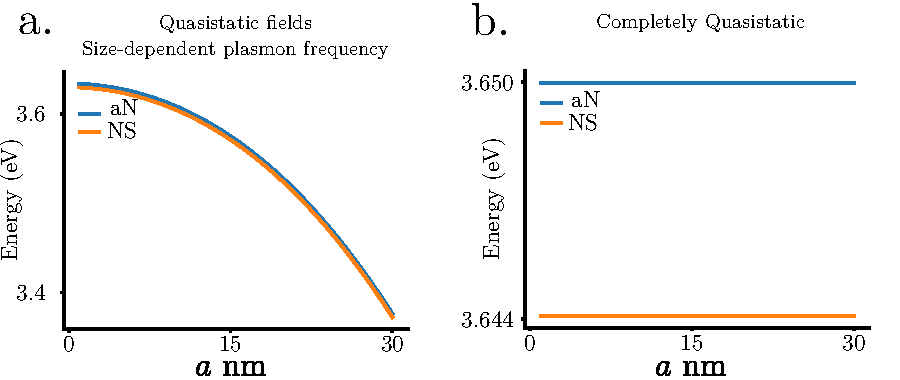
\includegraphics{qs_limit.pdf}
\caption{Resonance energies of the aN and NS modes of the 2-mer computed using (a) static fields with size-dependent $\omega_{\textrm{sp}}$ and (b) static fields and single MNP plasmon frequencies. In (a), the aN and NS energies decrease uniformly without crossing as a function of $a$. In (b), the mode energies do not decrease at all with increasing $a$, showing that retardation effects are necessary to model mode switching.}
\label{qs_limit}
\end{centering}
\end{figure}

An important question to ask is why it should be obvious that retardation effects are the cause of the mode switching seen in Chapter 3. If the mathematical explanation is not satisfying, it may help to investigate the impact of taking the quasistatic limit on the spectral order. Fig. \ref{diff_scale} does just that, in the case where just the fields are static (a), and in the case where both the fields and $\omega_{\textrm{sp}}$ lack size-dependence (b). Clearly, in the quasistatic approximation, the modes do not cross.

\newpage
\begin{figure}
\begin{centering}
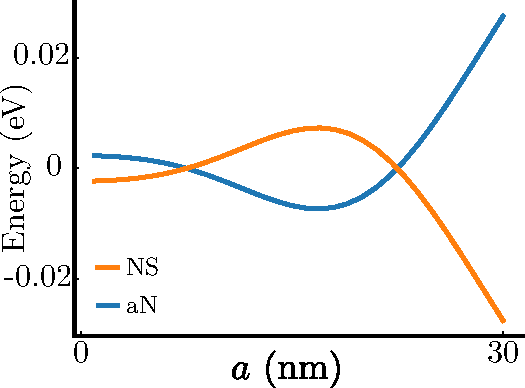
\includegraphics{eig_diff_scale.pdf}
\caption{Relative difference of the NS and aN mode energies from their average with increasing $a$. This shows much more clearly that the modes do change order and allows for the quantification of the splitting. The splitting at $a = 1$ nm is less than 0.01 eV, while at $a = 30$ nm it is nearly 0.06 eV.}
\label{diff_scale}
\end{centering}
\end{figure}

It also may be instructive to make sure that the curves in Fig. [look this up!] are actually crossing, and to quantify their splitting. Each curve's realtive difference from their average is plotted in Fig. \ref{diff_scale} in order to show that the modes do in fact switch order. The splittings are quite small, meaning that to see this splitting in an experiment a high-resolution instrument or spatio-specific method would be necessary.


\begin{figure}
\begin{centering}
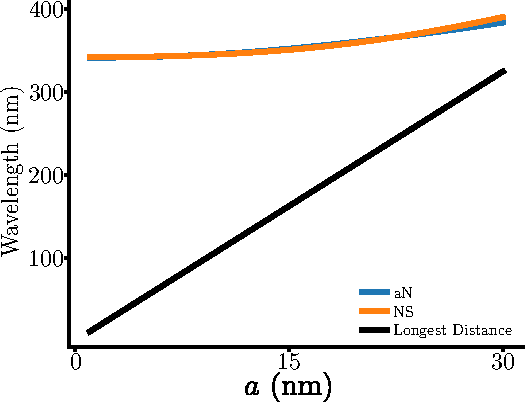
\includegraphics{length_comparison_scale.pdf}
\caption{Computed resonant wavelength for the NS and aN modes of the 2-mer, compared with the diagonal length of the oligomer. The modes cross at $a = 7$ nm, at which size the oligomer is about one quarter of the optical wavelength. This conflicts with the common ``half-wavelength'' rule of thumb.}
\label{scale_wavelength_comp}
\end{centering}
\end{figure}


Another interesting question is when the quasistatic approximation actually breaks down. The commonly reported rule of thumb is that the approximation is good for MNPs smaller than half a wavelength of the light used to interrogate them. However, this seems to break down for clusters that store large amounts of energy in their magnetic fields, as shown in Fig. \ref{scale_wavelength_comp}. Here, we compare the resonant wavelength $\lambda = 2\pi c/\omega$ to the ``longest distance'' in the oligomer, specifically its diagonal length.


\begin{figure}
\begin{centering}
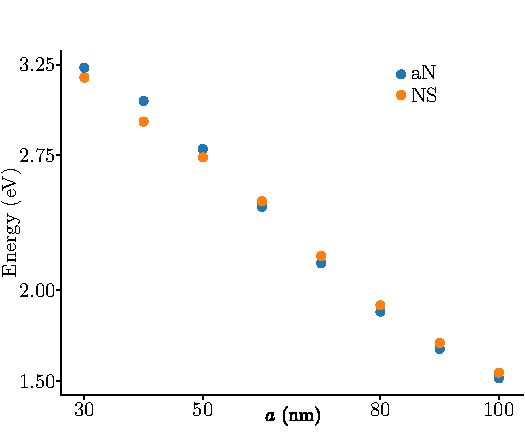
\includegraphics{bigger_particles.pdf}
\caption{Resonance frequencies of the NS and aN modes of the 2-mer for values of $a$ from 30 to 100 nm in increments of 10 nm. Between $a=50$ and $a=60$ nm, the modes cross a third time. Note that the splitting between the modes remains quite small with size. This would likely prevent any but the most highly-resolved experiments from detecting these modes.}
\label{bigp}
\end{centering}
\end{figure}


The modes continue to cross at larger MNP sizes, though the experimental practicality of oligomers of these sizes is unclear. It is likely that once the MNPs get large enough, their plasmon resonances get so broad as to make any magnetic resonances unresolvable. However, with theoretical approaches we can ask what happens when the particles do get bigger, and those results are shown in Fig. \ref{bigp}. 

\subsection{Parameter: interparticle spacing}


\begin{figure}
\begin{centering}
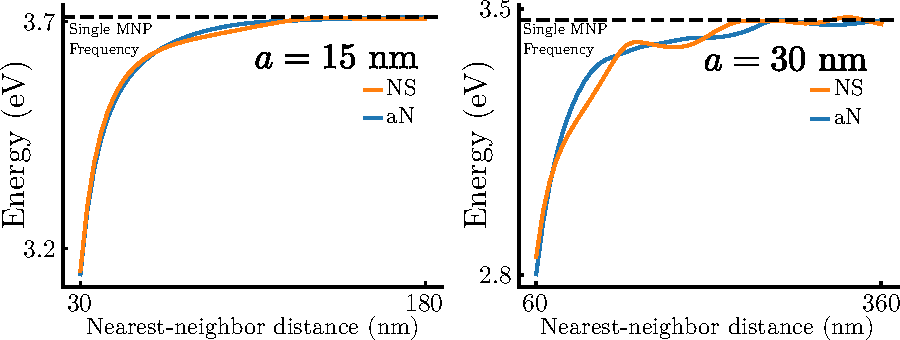
\includegraphics{spacing_2mer.pdf}
\caption{Resonance energies of the aN and NS modes of the 2-mer with respect to increasing interparticle distance for fixed $a=15$ nm (a) and $a=30$ nm (b). Note that with increasing separation, the resonance energies tend towards the single MNP plasmon frequency. In other words, the interaction energy goes to 0 as predicted by Eq. [look this up!]. Additionally, the collective energies oscillate about each other, contributing to multiple mode switches.}
\label{spacing_eig}
\end{centering}
\end{figure}


Another tunable parameter of experimental interest is the interparticle spacing (at constant $a$). Recent studies have shown the utility of using DNA or organic polymers as a means to link MNPs together and change, in real time, their interparticle spacing and conformation\cite{DanLuo2009,NaLiu2017,Ginger2017}. Here, we imagine linking the MNPs of the 2-mer into a constant configuration, and varying the interparticle distance uniformly, from 0 radii to 10 radii. Fig. \ref{spacing_eig} shows the impact of increasing the interparticle spacing at fixed radius on the magnetic modes of the 2-mer. Specifically, we choose $a=15$ nm (a) and $a=30$ nm (b).


\begin{figure}
\begin{centering}
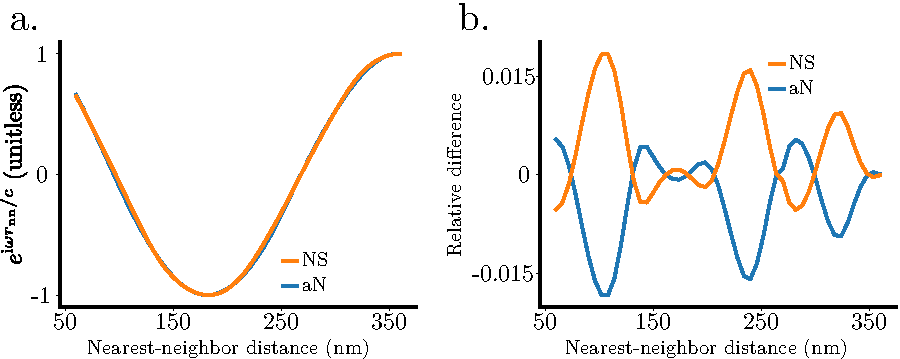
\includegraphics{diff_avg_space.pdf}
\caption{The exponential term from Eq. [look this up!] computed for the NS and aN modes of the 2-mer with increasing interparticle separation (a) and the relative difference between the exponential terms for each mode (b). This shows more clearly that the mode crossings, though exhibiting small splittings, are due to the exponential term in the dipolar electric field.}
\label{diff_avg_space}
\end{centering}
\end{figure}


The wiggles in the resonant frequencies are small, and thus the crossings are hard to distinguish. According to Chapter 3, the primary cause of mode-switching is the exponential term in Eq. [look this up!]. Fig. \ref{diff_avg_space} shows, for $a=30$ nm, the value of the exponential term for each mode as a function of the interparticle separation (a), and the relative difference between the exponential terms for each mode (b). This shows much more clearly that the modes do in fact cross.

\begin{figure}
\begin{centering}
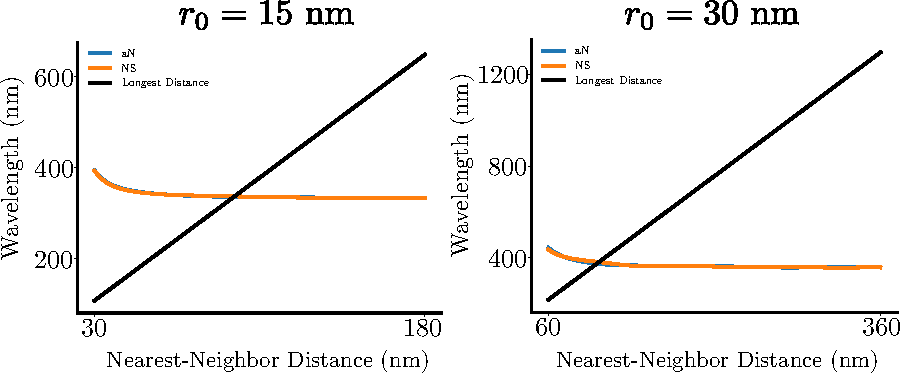
\includegraphics{length_comp_sapcing.pdf}
\caption{The resonance wavelength computed for the NS and aN modes of the 2-mer with increasing interparticle spacing and compared to the longest distance in the system for a radius of 15 (a) and 30 (b) nm. Note that in both cases, the oligomer very quickly becomes much larger than an optical wavelength.}
\label{length_space}
\end{centering}
\end{figure}


Again, how does this compare to commonly referenced size constraints on the quasistatic approximation? Fig. \ref{length_space} compares the resonant wavelength of each mode to the ``longest distance'' in the oligomer.


\section{Towards negative index metamaterials}

Consider a 1-mer of six MNPs arranged at the vertices of a regular hexagon. Such a cluster has both a collective magnetic mode and a collective electric mode. We know from the introduction that electric resonances occur when the permittivity ($\varepsilon(\omega)$) is negative. Here we will show that magnetic modes occur when the collective permeability ($\mu_{\textrm{eff}}(\omega)$) is negative. Materials that are double-negative, that is, having negative permittivity and permeability, exhibit a negative index of refraction. The approach here was first presented by Al\'{u} and Engheta in 2006[citation needed], and we adapt it for our purposes.

Consider the magnetic mode of the 1-mer of radius $R$ driven by an incident magnetic field $\textbf{H} = H_0\hat{\textbf{z}}$ and electric field $\textbf{E}_0 = \textrm{i}\omega\mu_0RH_0/2\hat{\phi}$. This is sets up a dipole moment on each MNP
\begin{equation}
\textbf{d}_i = d\hat{\phi}_i = \alpha_{\textrm{sp}}E_{\textrm{loc}}\hat{\phi}_i
\label{dipole_moment_1}
\end{equation}
where $E_{\textrm{loc}}\hat{\phi} = \textbf{E}_0 + \sum_{i\neq j}\textbf{E}_{ij}$ and $\textbf{E}_{ij} = \boldsymbol{\Lambda}_{ij}\cdot\textbf{p}_j$. We want to find the induced dipole moment on each MNP from the influence of the incident field and each other MNP. Plugging in the definitions of the field, this dipole moment is
\begin{equation}
d\hat{\phi}_i = \alpha_{\textrm{sp}}\left(\frac{\textrm{i}\omega\mu_0RH_0}{2}\hat{\phi}_i + d\sum_{i\neq j}\boldsymbol{\Lambda}\cdot\hat{\phi}_j\right).
\label{dipole_moment_2}
\end{equation}
Projecting out the $\hat{\phi}$-dependence and manipulating the terms, the induced dipole moment on each MNP takes the form
\begin{equation}
d = \alpha_{\textrm{sp}}\left(\frac{\textrm{i}\omega\mu_0RH_0}{2\left[1 - \alpha_{\textrm{sp}}\sum_{i\neq j}\hat{\phi}_i\cdot\boldsymbol{\Lambda}_{ij}\cdot\hat{\phi}\right]}\right).
\label{dipole_moment_3}
\end{equation}

Now that we have the individual dipole moments, we still need to construct the permeability. We will go through a collective polarizability, starting by writing down the collective magnetic dipole moment. The magnetic dipole moment of any current distribution is $\boldsymbol{mu}_H = (\textrm{i}\omega/2)\int d^3r\textbf{r}\times\textbf{J}$. For a ring of $n$ particles, that magnetic dipole moment is
\begin{equation}
\boldsymbol{\mu}_H = -\frac{\textrm{i}\omega pnR}{2}\hat{\textbf{z}} = \alpha_{M}\textbf{H}_0.
\label{mag_dip_1}
\end{equation}
where we have also related it to the magnetic polarizability. Making the assumption that $\alpha_M = \boldsymbol{\mu}_H/\textbf{H}_0$ and plugging in all of the previous definitions, we arrive at the magnetic poalrizability
\begin{equation}
\alpha_M = \frac{N(kR)^2}{4\varepsilon_0}\left[\alpha_{\textrm{sp}}^-1 - \sum_{i\neq j} \hat{\phi}_i\cdot\boldsymbol{\Lambda}_{ij}\cdot\hat{\phi}_j\right].
\label{alpha_mag}
\end{equation}
This quantity represents how easy or hard it is to push on the magnetic dipole of the 1-mer. From here, we get to the permeabilty through effective medium theory, noting that $N_d\alpha_M = 3\mu_0[(\mu_eff-\mu_b)/(\mu_eff-2\mu_b)]$ where $N_d$ is the number density of oligomers and $\mu_b$ is the background permeability (nearly 1 for most materials). Solving for the effective permeabilty results in
\begin{equation}
\mu_{\textrm{eff}} = \mu_0\left(1+\frac{1}{N_d^{-1}\alpha_M^{-1}-1/3}\right).
\label{mu_eff}
\end{equation}

We now need to find not the single MNP permittivity, but rather the collective permittivity of the collective electric dipole moment of the 1-mer. We will follow the same approach as previosuly, except now the incident electric field is $\textbf{E}_0 = E_0\hat{\textbf{y}}$. Doing everything we did before, we arrive at the effective electric permittivity
\begin{equation}
\varepsilon_{\textrm{eff}} = \varepsilon_0\left(1+\frac{1}{\varepsilon_0N_d^{-1}\alpha_E^{-1}-1/3}\right).
\label{eps_eff}
\end{equation}

We can now compute the index of refraction. Consider, as an example, the case where both $\mu_{\textrm{eff}}$ and $\varepsilon_{\textrm{eff}}$ are negative, then the index of refraction is $n = \sqrt{\mu_{\textrm{eff}}\varepsilon_{\textrm{eff}}} = i\sqrt{\mu_{\textrm{eff}}}i\sqrt{\varepsilon_{\textrm{eff}}} < 0$. In Fig. \ref{n_plot}, we have computed the frequency- and size-dependent index of refraction of both the 1-mer (a) and 2-mer (b). The blue regions of the graph are those frequencies and sizes where the clusters have a negative index of refraction. Future applications of this property will require ways to widen the frequency window of the negative-index region, perhaps by tailoring systems to have multiple electric and magnetic resonances.


\begin{figure}
\begin{centering}
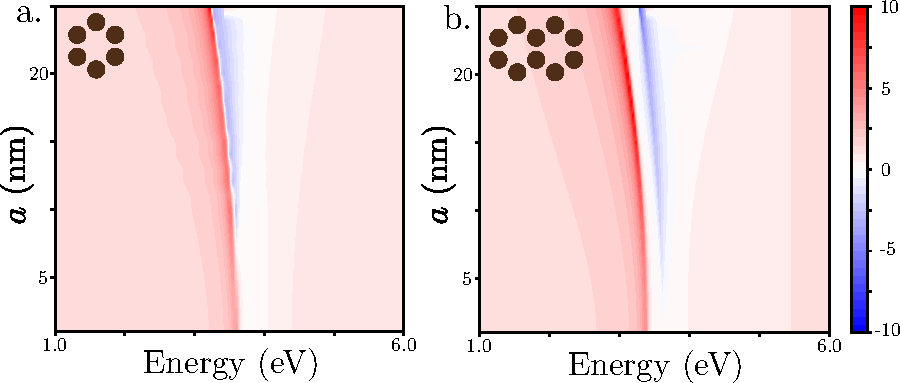
\includegraphics{contour_n_plot.pdf}
\caption{Collective index of refraction as a function of increasing $a$ and incident photon energy for two unit cells: a 1-mer (a) and a 2-mer (b). The red regions correspond to positive index of refraction, the blue regions correspond to negative index of refraction, and the white regions show an index of refraction near zero [look up n near zero materials]. These plots show that using size can be used as a parameter to tune the range of optical frequencies in which a material has a negative index of refraction. This can serve to make materials that transmit specific or all colors of light.}
\label{n_plot}
\end{centering}
\end{figure}

%
% ==========   Bibliography
%
%\nocite{*}   % include everything in the uwthesis.bib file
\bibliographystyle{ieeetr}
\bibliography{references}
%

\end{document}
